\chapter{Umsetzung des Prototyps}\label{sec:realisation}

Nachdem in Kapitel \ref{sec:concept} die Konzeption der Anwendungen dargestellt wurde, folgt in diesem Kapitel die Beschreibung der praktischen Umsetzung.

Zunächst wird die Ausgangssituation erläutert, wie sie sich aus dem vorangegangenen Projekt ergab. Anschließend erfolgt eine Übersicht der verwendeten Technologien. Darauf aufbauend werden die entwickelten Anwendungen im Detail vorgestellt. Abschließend werden zentrale Herausforderungen und Probleme beschrieben, die im Verlauf der Umsetzung auftraten.

\section{Ausgangssituation}

In der vorangegangenen Arbeit wurde ein erstes funktionsfähiges \ac{MVP} der Spielidee realisiert das sich aus drei Hauptkomponenten zusammensetzt. Die Spielanwendung für den Player wurde mithilfe der Game Engine Unity umgesetzt. Das Spielgeschehen des Watchers wurde hingegen als Webanwendung auf Basis des Vue3-Frameworks realisiert. Für die Kommunikation zwischen beiden Anwendungen wurde ein WebSocket-Server auf Grundlage von Express.js (Auf Basis von Node.js) entwickelt. Dieser Server steht zusätzlich in Verbindung mit einer MongoDB-Datenbank, in der die Fortschritte einzelner Spielsessions gespeichert werden.

Die Anwendungen des Players und des Watchers fungieren in diesem System als visuelle und interaktive Frontend, die auf Nutzereingaben reagieren. Diese Eingaben werden an den Server übermittelt, der sie zur Laufzeit verarbeitet und bei Bedarf persistent in der Datenbank speichert.

\subsection{Aufbau der Ausgangssituation}

Im Softwaredesign wurde in diesem Zusammenhang häufig auf das \ac{MVC} zurückgegriffen (vgl. \citealp{GlossarWiki:Reenskaug:1979a}). Das Modell (Model) definiert die Datenstruktur der Anwendung und enthält die zugrunde liegende Information. Bei einer Zustandsänderung benachrichtigt das Modell die jeweiligen Views, sodass die Darstellung der Daten entsprechend aktualisiert wird. In einigen Implementierungen wird zusätzlich auch das Controller über Änderungen informiert.

Die View legt fest, wie die Daten visuell präsentiert werden. Der Controller wiederum ist für die Bearbeitung der Nutzereingabe verantwortlich. Er nimmt die Änderungen aus der View entgegen und übermittelt sie entweder an das Modell oder direkt zurück an die View (vgl. \citealp{mills_mvc_2025}, Abbildung \ref{fig:mvc-diagramm}).

\begin{figure}[ht]
\centering
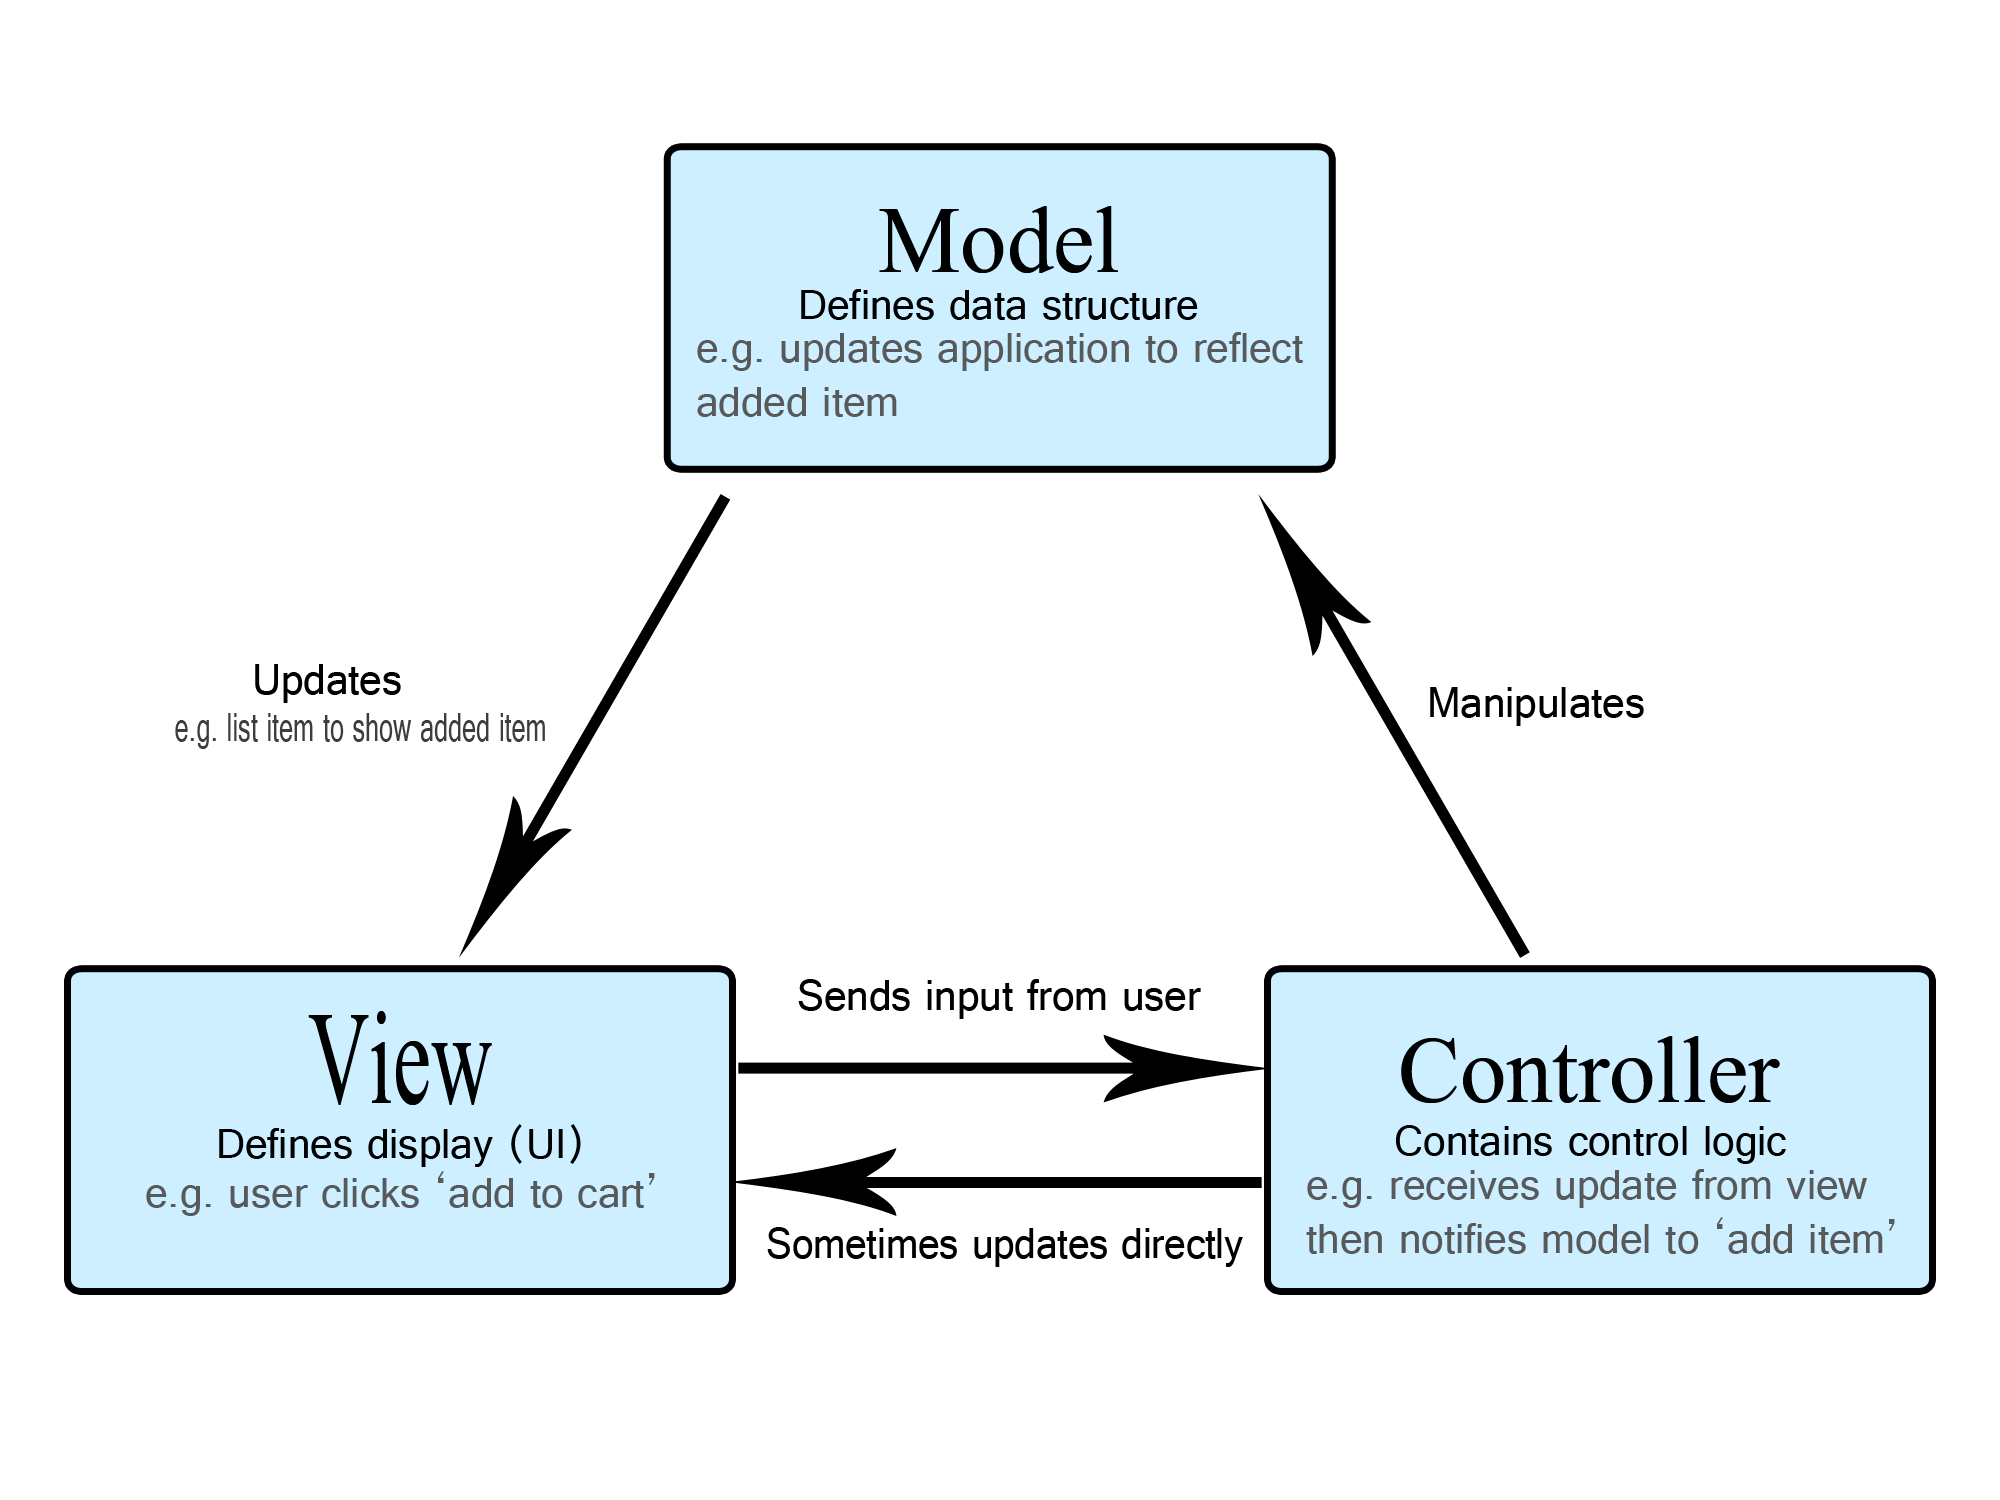
\includegraphics[width=1\linewidth]{content/pictures/mvc-architecture.png}
\caption{\ac{MVC} Beispiel-Diagramm (Quelle: \cite{mills_mvc_2025})}
\label{fig:mvc-diagramm}
\end{figure}

Innerhalb der Systemarchitektur übernehmen die MongoDB-Datenbank sowie bestimmte Klassen des WebSocket-Servers die Rolle des Modells. Sie verwalten die zentralen Anwendungsdaten und deren Persistenz. Die verschiedenen WebSocket-Nachrichtenendpunkte fungieren als Controller. Sie verarbeiten eingehende Nachrichten, koordinieren die Datenflüsse zwischen Modul und View und steuern die Anwendungslogik. Die \say{Frontends} der Watcher- und Player-Anwendungen bilden die Views des \ac{MVC}-Design-Patterns und dienen der Darstellung sowie Interaktion mit dem Nutzer.

\subsection{Beitreten einer Session}

\begin{figure}[ht]
\centering
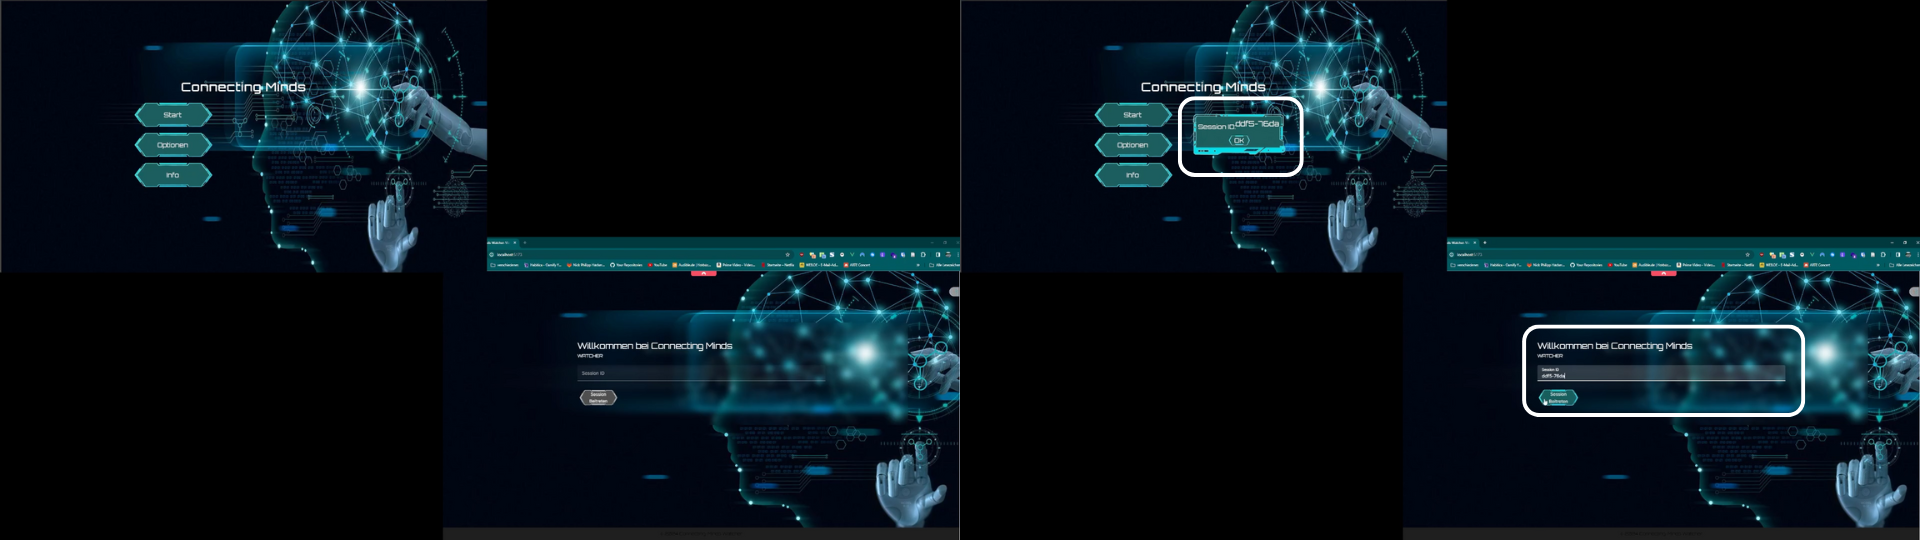
\includegraphics[width=1\linewidth]{content/pictures/Login_Login_by_ID.png}
\caption{Startbildschirme der Player und Watcher Anwendung (Quelle: eigene Darstellung)}
\label{fig:old-logins}
\end{figure}

Abbildung \ref{fig:old-logins} zeigt den bereits im früheren Prototyp entwickelten Startbildschirm, über den der Player eine neue Spielsession starten (linkes Bild, oben links) und der Watcher dieser beitreten kann (linkes Bild, unten rechts). Nachdem der Player eine Session erstellt hat, erhält er vom WebSocket-Server eine Rückmeldung mit der dazugehörigen Session-ID (rechtes Bild, oben links). Diese ID muss er dem Watcher mitteilen, damit dieser der entsprechenden Session beitreten kann (rechtes Bild, unten rechts).

\subsection{Einführung in die Anwendungen}

\begin{figure}[ht]
\centering
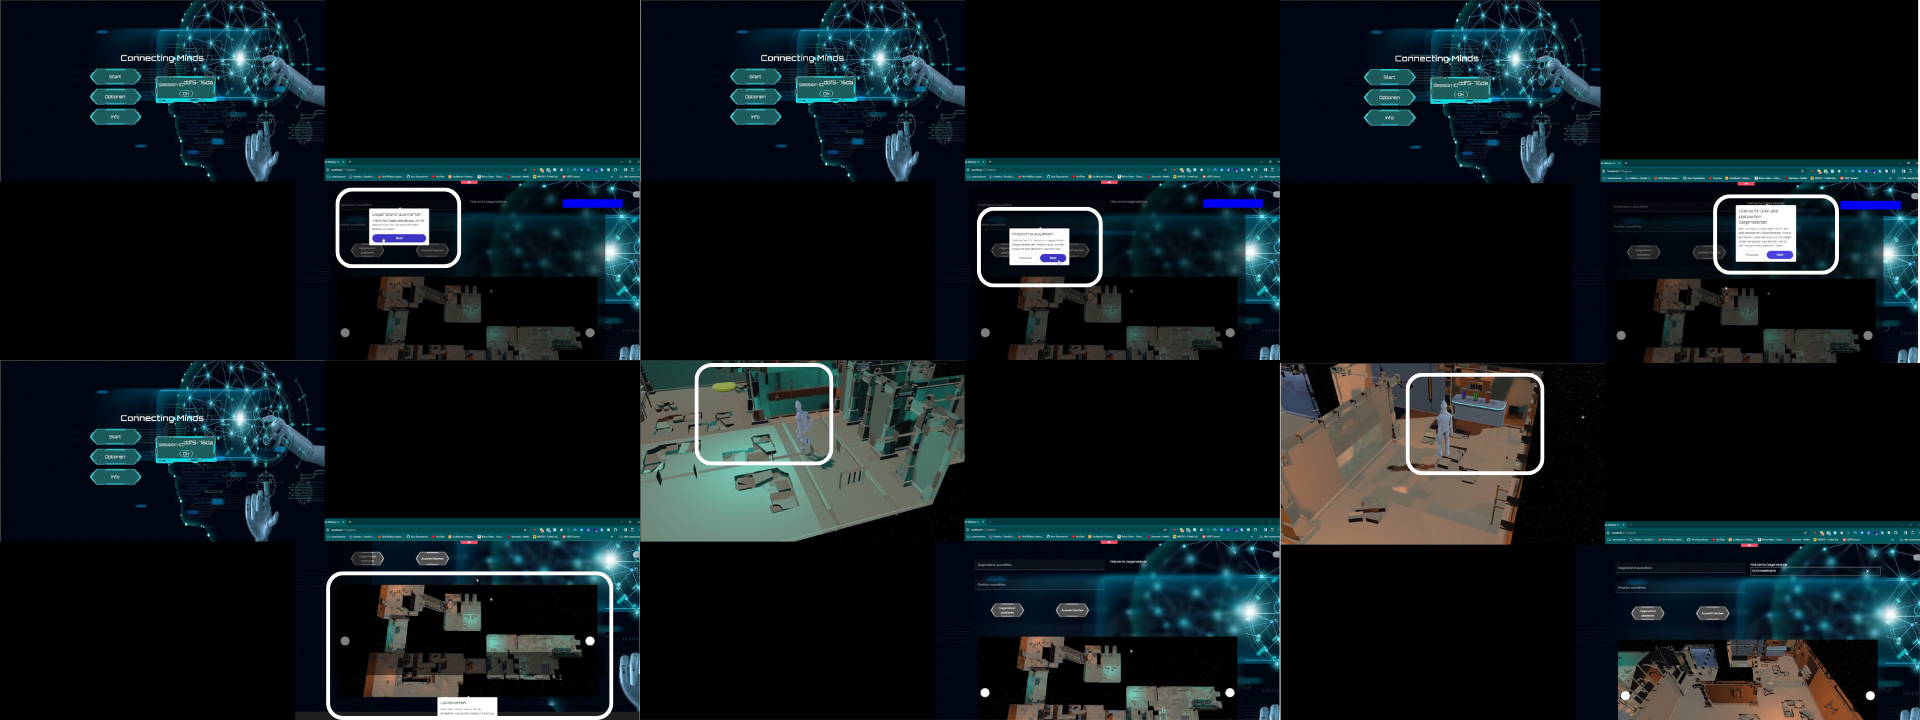
\includegraphics[width=1\linewidth]{content/pictures/Introduction.png}
\caption{Einführung in die Anwendung des Players und Watchers (Quelle: eigene Darstellung)}
\label{fig:old-introductions}
\end{figure}

Abbildung \ref{fig:old-introductions} zeigt die Einführung der beiden Anwendungen in die Spielwelt. Zu Beginn erhält der Watcher verschiedene Tooltips, die ihm die Grundfunktionen seiner Anwendung erläutern (vgl. erstes bis drittes Bild in der ersten Zeile und linkes Bild in der zweiten Zeile; jeweils in weiß umrandet im rechten Bildelement). Die Anwendung des Watchers umfasst zwei Dropdown-Menüs, über die Gegenstände und deren Positionen ausgewählt werden können (erste Zeile, Bilder links und und in der Mitte), eine Lister aller aktuell platzierten Objekte (erste Zeile rechts Bild), welche einzeln wieder entfernt werden können, sowie eine Top-Down-Ansicht der Spielwelt, in der sich der Player befindet (zweite Zeile, linkes Bild). 

Der Player steuert seinen Avatar durch Antippen der gewünschten Position auf dem Bildschirm (zweite Reihe mittlere Bild, linkes Bildelement). Zusätzlich kann er die Kamerahöhe in Relation zur Spielfigur durch vertikale Wischbewegungen (Swipes) anpassen, wodurch sich die Perspektive innerhalb eines bestimmten Rahmens verändert.

Um das gemeinsame Spielziel zu erreichen, müssen Player und Watcher kooperieren und gemeinsam Hindernisse in der Spielwelt überwinden. Ein solches Rätselelement, das im Zusammenspiel gelöst werden muss, ist im weiß umrandeten Bereich des linken Bildes in der zweiten Zeile dargestellt.

\subsection{Lösen von Rätseln}

Wie wurden im ursprünglichen Prototyp die einzelnen Rätsel gelöst und durch wen erfolgte dies?

\begin{figure}[ht]
\centering
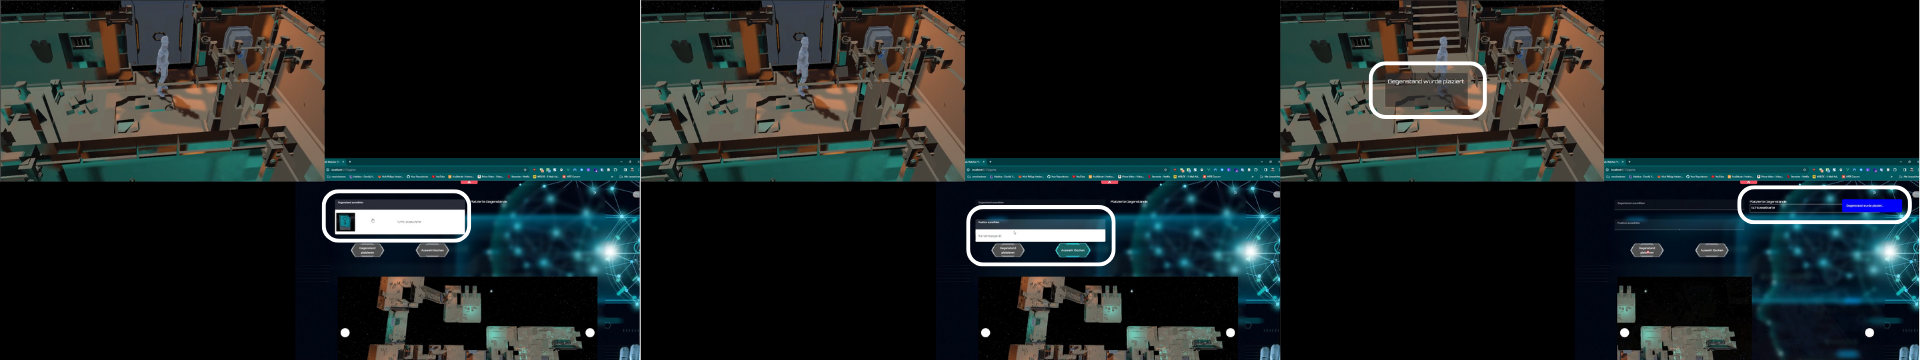
\includegraphics[width=1\linewidth]{content/pictures/HowToSolve.png}
\caption{Vorgang des Lösens von Rätseln (Quelle: eigene Darstellung)}
\label{fig:old-solving-riddle}
\end{figure}

Im früheren Prototyp lag die alleinige Verantwortung für die Lösung der Rätsel beim Watcher. Dieser war dafür zuständig, die richtigen Gegenstände an den jeweils korrekten Zielpositionen zu platzieren. Sobald der Player in der Spielwelt auf eine Absperrung stieß, musste er seine Beobachtungen verbal schildern, um dem Watcher Hinweise darauf zu geben, welche Gegenstände an welchen Positionen benötigt werden.

Der Lösungsprozess verlief wie folgt. Zunächst wählte der Watcher über das Dropdown-Menü für Gegenstände den entsprechenden Gegenstand aus (vgl. Abbildung \ref{fig:old-solving-riddle}, linkes Bild, rechtes Bildelement). Anschließend wählte er eine Zielposition aus einer vordefinierten Liste von Platzierungsoptionen, die in den aktuell aktiven Abschnitten der Spielwelt verfügbar waren (vgl. mittlere Bild, rechts Bildelement). Über den Button \say{Gegenstand platzieren} (linker Button) wird der Gegenstand in die Spielwelt des Players eingefügt.

Nach erfolgreicher Platzierung erhielten sowohl Player als auch Watcher eine visuelle Rückmeldung durch das System (vgl. rechts Bild, beide weiß Umrandeten Elemente). Zusätzlich wurde der neu platzierte Gegenstand automatisch in die Liste der aktuell vorhandenen Gegenstände auf der rechten Seite der Watcher-Anwendung übernommen (rechtes Bild, rechtes Bildelement). 

\subsection{Freischalten von Gegenständen und Positionen}

Sobald ein Rätsel durch das Platzieren der richtigen Gegenstände gelöst wurde, erhielten sowohl der Player als auch der Watcher eine Rückmeldung darüber, dass neue Gegenstände freigeschaltet wurden (vgl. Abbildung \ref{fig:old-unlock-system}, erste Reihe linkes Bild, weiß eingekreist). 

\begin{figure}[ht]
\centering
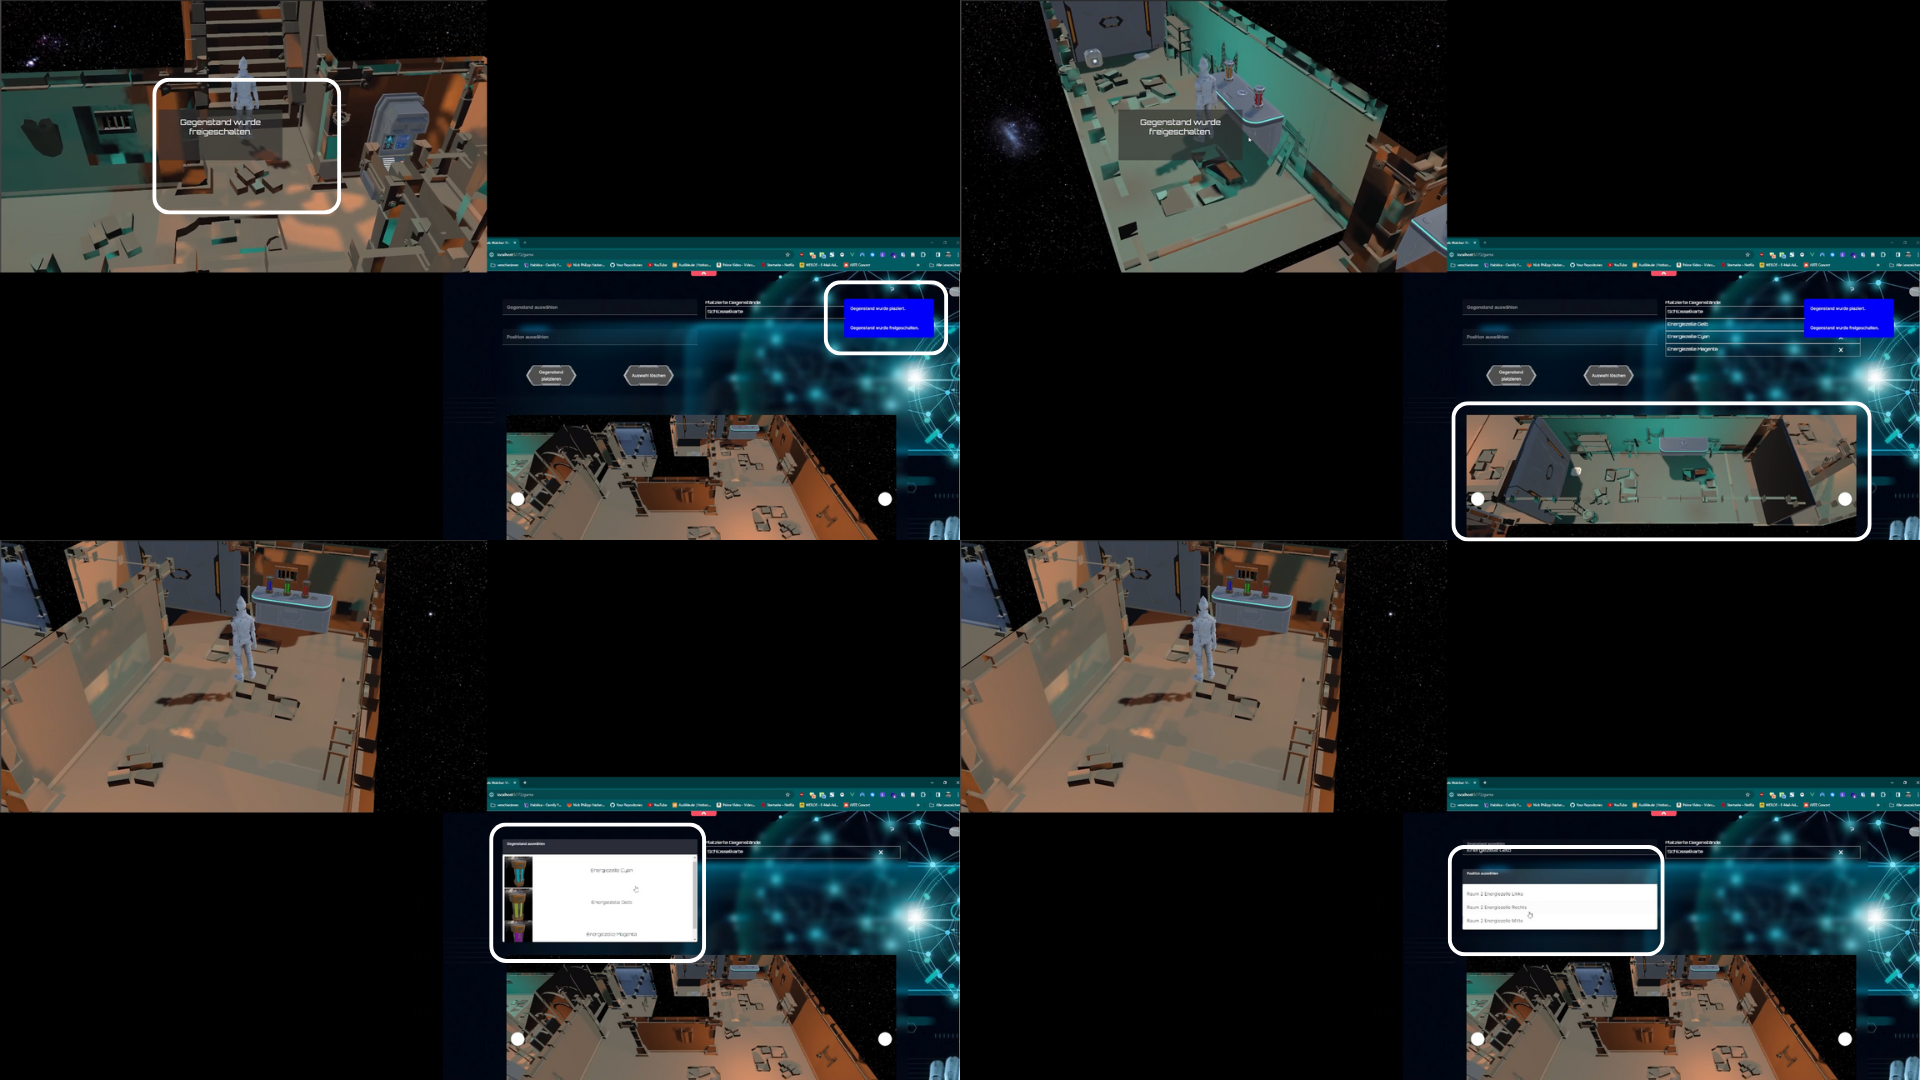
\includegraphics[width=1\linewidth]{content/pictures/UnlockMore.png}
\caption{Freischalten neuer Gegenstände (Quelle: eigene Darstellung)}
\label{fig:old-unlock-system}
\end{figure}

Wenn durch das Lösen des Rätsels ein Hindernis entfernt und ein neuer Bereich der Spielwelt zugänglich gemacht wurde, aktualisierte sich der Bilder-Slider in der Watcher-Anwendung automatisch und wechselte zur aktuell freigeschalteten Ansicht. Der Slider zeigt dem Watcher alle derzeit verfügbaren Abschnitte der Spielwelt  (vgl. Abbildung \ref{fig:old-unlock-system}, erste Reihe, rechtes Bild, weiß umrandet). 

Mit dem Zugang zu neuen Spielabschnitten werden nicht nur zusätzliche Gegenstände freigeschaltet, sondern auch weitere vordefinierte Zielpositionen, auf denen diese platziert werden können. Diese neuen Optionen erscheinen im Watcher-Interface in den Dropdown-Menüs für Gegenstände und Positionen (vgl. Abbildung \ref{fig:old-unlock-system}, zweiten Reihe, beide Bilder, jeweils weiß umrandet). 

\subsection{Aspekte zum Überarbeiten}

In diesem Kapitel werden jene Aspekte des ursprünglichen Prototyps dargestellt, die in der Umsetzung als unzureichend identifiziert wurden und im Rahmen der Weiterentwicklung im neuen Prototyp überarbeitet werden sollen.

\paragraph{Backfaces}

In den zuvor dargestellten Abbildungen \ref{fig:old-logins} bis \ref{fig:old-unlock-system} ist zu erkennen, dass die Wände der Spielwelt, in der sich der Player befindet (jeweils das linke Bildelement), eine ungewöhnliche und falsche Darstellung aufweisen. Dies liegt daran, dass die verwendeten Raumelemente ursprünglich für eine Kameraperspektive aus dem Inneren des Raums konzipiert wurden. Um eine konkrete Darstellung zu gewährleisten, wäre für diesen Aufbau eine First-Person-Kamera notwendig.

\begin{figure}[ht]
\centering
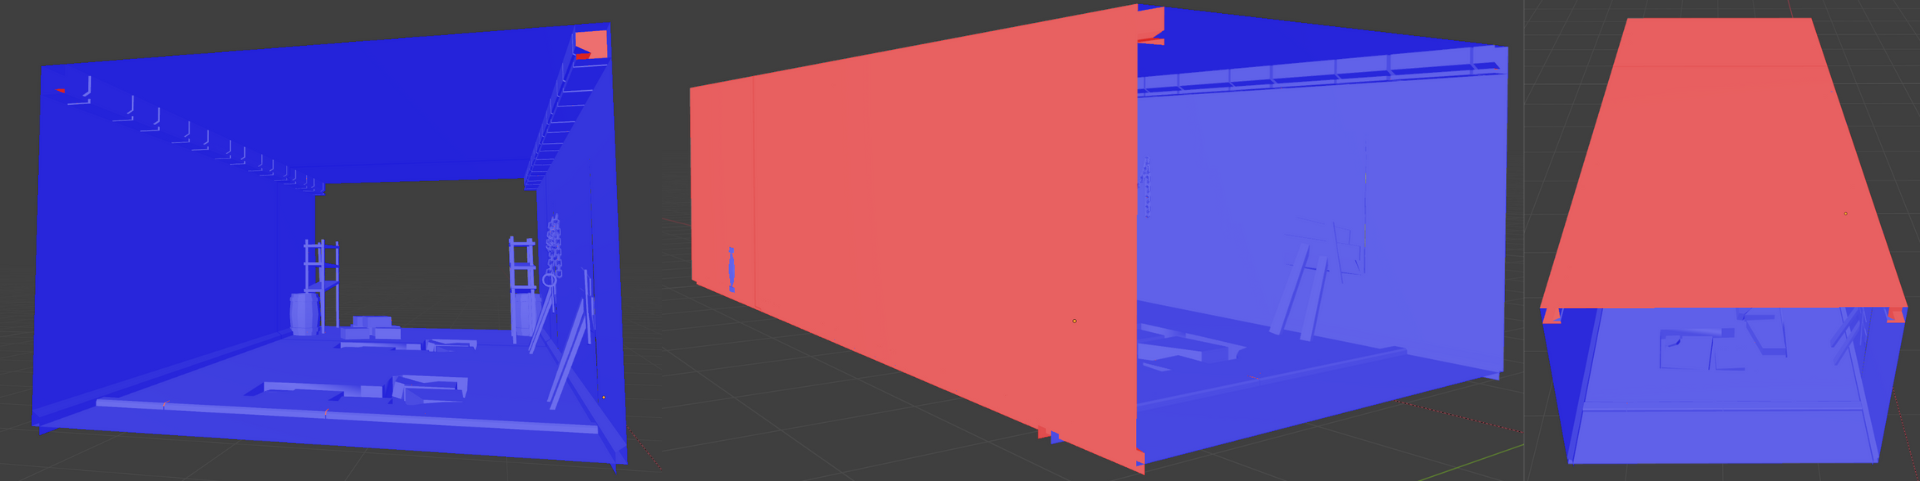
\includegraphics[width=1\linewidth]{content/pictures/Backfaces.png}
\caption{Fehlende Rückwand-Oberflächen in den Raummodellen (Quelle: eigene Darstellung), (Modell von \cite{alasl_autolevel_2022})}
\label{fig:missing-backfaces}
\end{figure}

Abbildung \ref{fig:missing-backfaces} verdeutlicht, dass Rückseitenflächen bei der aktuellen Modellierung fehlen. Die blauen Flächen kennzeichnen Oberflächen, deren Normalvektoren in Richtung der Kamera zeigen und somit von der Game Engine gerendert werden können. Die roten Flächen hingegen sind Rückseiten, deren Normalvektoren von der Kamera wegzeigen und die daher standardmäßig nicht dargestellt werden.

Zur Behebung dieses Problems bestehen grundsätzlich zwei Lösungsansätze. Entweder wird in der Materialkonfiguration der betroffenen Objekte bidirektionales Rendering aktiviert, oder das Modell wird so angepasst, dass es für jede Betrachtungsrichtung eigene Flächen mit entsprechend ausgerichteten Normalen enthält.

Für die beabsichtige Nutzung in einem Spiel mit Top-Down-Perspektive ist es darüber hinaus erforderlich, die Decken der Räume zu entfernen, da diese aus der gewählten Kameraperspektive nicht sichtbar sind und die Sicht auf relevante Elemente der Spielwelt beeinträchtigen würden.

\paragraph{Steuerung des Avatars}

Im vorangegangenen Prototyp wurde der Gestaltung der Spielsteuerung mittel Touch-Input nur geringe Aufmerksamkeit geschenkt. Die im Projekt zu Beginn eingesetzte Standardsteuerung des verwendeten Unity-Assets von \cite{alasl_autolevel_2022} unterstützte ausschließlich Maus- und Tastatureingaben. Die Fortbewegung innerhalb der Spielwelt erfolgte die Steuerung der Kamera über die Tastatur, ähnlich wie in \ac{RTS}-Spielen, während ein Klick mit der linken Maustaste eine Bewegung des Avatars zur angeklickten Position auslöste.

Eine Steuerung über Touch-Eingaben, etwa an einem Touchscreen-Monitor oder Fernsehgerät, war in der ursprünglichen Implementierung des Beispielprojekts nicht vorgesehen und musste nachträglich ergänzt werden. Das Asset von \cite{alasl_autolevel_2022} nutzt das Cinemachine-Kamerasystem, wodurch einige mausbasierte Kamerasteuerungen bereits vorimplementiert waren (vgl. \citealp{unity_technologies_about_2017}). Eine spezifische Touch-Steuerung hingegen fehlte vollständig.

Die nachträglich hinzugefügte Touch-Eingabe orientierte sich nicht nach etablierten Standards für Touch-Interfaces, wie sie bspw. von \cite{reinhard_augmented_2022} vorgeschlagen werden (vgl. \citealp[S. 64ff]{reinhard_augmented_2022}),
stattdessen wurde eine eigens entwickelte Lösung implementiert, die jedoch nicht denselben Bedienkomfort wie die Maussteuerung bieten konnte.

\paragraph{Interaktion mit der Spielwelt}

Sowohl in der Anwendung des Players als auch in der Watchers bestanden bislang nur sehr eingeschränkte, teils gar keine Interaktionsmöglichkeiten mit der Spielwelt. In der Player-Anwendung beschränkte sich die Interaktion auf das Navigieren innerhalb der Spielumgebung. Die Watcher-Anwendung verfügte hingegen über keinerlei Funktionalitäten im direkten Bezug auf die Spielwelt. Die Interaktion beschränkte sich auf die Menüführung, über die Sitzungsdaten verwaltet werden konnten.

Für den zukünftigen Prototyp ist es daher essenziell, die zentralen Kernfunktionen zu integrieren, die eine vertiefte Interaktion mit der Spielwelt ermöglichen. Nur so kann das interaktive Zusammenspiel zwischen Player und Watcher gewährleistet werden.

\paragraph{Sonstiges Feedback aus den Probandentests}
\begin{figure}[ht]
\centering
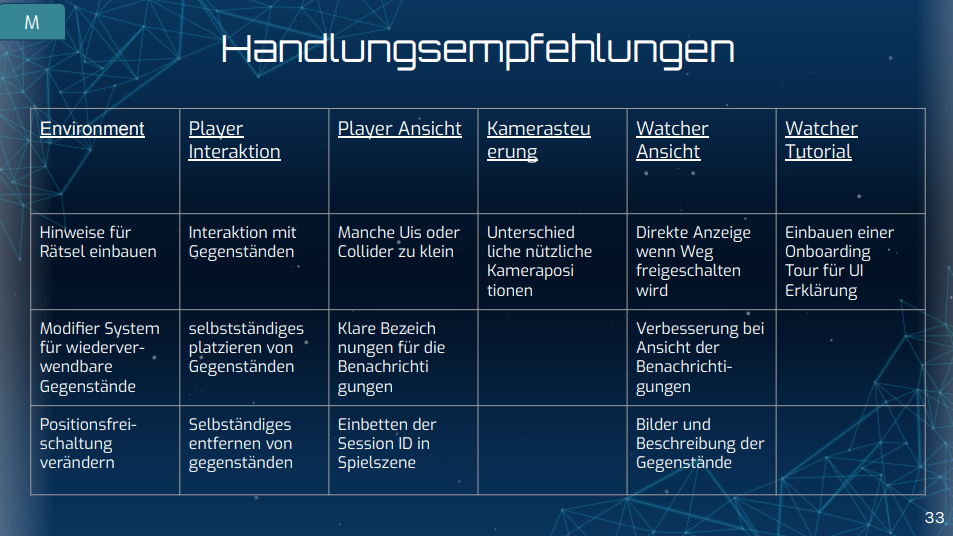
\includegraphics[width=1\linewidth]{content/pictures/Handlungsempfehlungen.PNG}
\caption{Handlungsempfehlungen des alten Prototyps (Quelle: eigene Darstellung aus der Abschlusspräsentation), (ganze Präsentation in Anhang \ref{sec:append_realisation_ausgangslage_presentation}: \nameref{sec:append_realisation_ausgangslage_presentation}, S. 33)}
\label{fig:recommended-action}
\end{figure}

Abbildung \ref{fig:recommended-action} stellt die in der vorangegangenen Arbeit formulierten Handlungsempfehlungen für den ursprünglichen Prototyp dar. Die Bereiche \say{Player Interaktion}, \say{Player Ansicht}, \say{Kamerasteuerung} sowie \say{Watcher Ansicht} wurden in den o. g. Abschnitten bereits thematisiert. Die Punkte \say{Environment} und \say{Watcher Tutorial} blieben bislang unberücksichtigt. Insbesondere das \say{Watcher Tutorial} wurde in der Weiterentwicklung des Prototyps nicht implementiert, da der konzeptionelle und technische Aufwand für die Erstellung eines integrierten Tutorials zur Einführung in die \ac{UI}-Elemente als zu hoch eingeschätzt wurde. Ein entsprechendes Tutorials müsste darüber hinaus auch für die Anwendung des Players vorgesehen werden, was den Entwicklungswand weiter erhöht hätte.

Im Folgenden wird der Fokus daher auf das Environment gelegt. Die Handlungsempfehlungen in Abbildung \ref{fig:recommended-action} beziehen sich auf das bestehende System des Prototyps, lassen sich jedoch abstrahieren und auf eine umfassendere Weiterentwicklung übertragen. Eine solche Weiterentwicklung würde neue Möglichkeiten zur Gestellung und Integration von Rätseln innerhalb der Spielwelt eröffnen. So könnten etwas Interaktionspunkte auf der Karte dynamisch und nicht mehr ausschließlich vordefiniert positioniert werden. Ebenso wäre es denkbar, bestehende Objekte in ihrer Funktionalität oder Erscheinung zu verändern, um neue Spielmechaniken zu ermöglichen. Diese Potenziale sollten bei einer zukünftigen Neugestaltung des Environments berücksichtigt werden, um die spielerische Tiefe und Varianz zu erhöhen.

\section{Verwendete Technologien}

In der folgenden Auflistung werden sämtliche externen Assets und Packages vorgestellt, die während der Entwicklung des Prototyps zum Einsatz kamen. Einige dieser Assets sind nicht in der Projekt-Registry aufgeführt, da sie zunächst in ein separates Testprojekt importiert, dort bearbeitet und anschließend als angepasste Submodule in das Hauptprojekt integriert wurden.

\subsection{Unity Editor Version 2022.3.45f1}
Der Prototyp wurde mit der 2022.3.45f1 \ac{LTS}-Version umgesetzt, da diese zum Start der Masterarbeit die aktuelle 2022 \ac{LTS}-Version war. Zwischenzeitlich wurde auch die 2023.2.20f1 (vgl. \citealp{unity_technologies_unity_2024}) ausprobiert. Da diese allerdings weder eine \ac{LTS}-Version noch zusätzlich im Package der Cinemachine ein Major-Update enthalten war und die Cinemachine einige Probleme mit sich führte, wurde eine stabile 20222-Version gewählt.

\subsection{Blender 4.3.2}
Blender dient als Bearbeitungstool für die 3D-Modelle aus den hinzugenommenen Unity Assets. Die aktuelle Version zu Projektstart war die 4.3.2 Version- welche über den gesamten Bearbeitungszeitraum verwendet wurde. Außerdem bietet Unity einen Blender Direktimport an, wodurch keine \ac{FBX} oder \ac{OBJ} Dateien aus den Blenderdateien exportiert und in Unity importiert werden mussten.

\subsection{NuGetForUnity 4.1.1}
NuGetForUnity ist ein für Unity entwickelter NuGet-Client (vgl. \citealp{microsoft_nuget_2010}) über den zusätzliche funktionale Pakete für Unity installiert werden kann (vgl. \citealp{mccarthy_glitchenzonugetforunity_2024}). Er war nötig, um ein nicht über Unity erworbenes Package in Unity nutzen zu können. Die aktuelle Version zum Bearbeitungsstart war die 4.1.1 Version, welche bis zum Ende genutzt wurde.

\subsection{Newtonsoft.Json 13.03}
Das erste Package, welches über NuGetForUnity installiert wurde ist Newtonsoft.Json, durch welches über den WebSocket übertragene JSON-Daten leicht deserialisiert und serialisiert werden können (vgl. \citealp{newton-king_jsonnet_2023}). Die aktuelle Version im NuGet-Paketverwaltungstool war die 13.03.

\subsection{WebSocketSharp-netstandard 1.0.1}
Derzeit gibt es einige Netzwerk-Integrationen für Unity, bspw. Mirror (vgl. \citealp{mirrornetworking_mirrornetworkingmirror_2025}) oder Netcode for GameObjects (vgl. \citealp{reeve_about_2025}). Durch die beiden Packages wäre jedoch die Netzwerk-Topologie starrer und die Entwicklung nach eigener Vorstellung wäre ebenfalls eingeschränkter. Daher wurde über NuGetForUnity das WebSocketSharp-netstandard Paket installiert, welches eine direkte Kommunikation mit einem WebSocket-Server ermöglicht (vgl. \citealp{pingman_tools_websocket-sharp_2017}), da bislang existierende Integration mit Unity nicht mehr unterstützt werden. Die derzeit installierte und zum Projektstart installierbare Version ist die 1.0.1.

\subsection{AI Navigation 1.1.5}
Da sich der Avatar des Players innerhalb der Spielwelt per Touch-Click auf den Bildschirm an die angeklickte Stelle bewegen soll, muss ein \ac{AI}-Agent eingebaut werden, der das Avatar Spielobjekt an die gewünschte Stelle bewegt. In Unity kann dafür das NavMesh System verwendet werden, welches ein Pathfinding-System implementiert, wodurch ein automatisiertes Bewegen eines Agents durch eine Zielposition integriert werden kann. Das Paket in Unity heißt \ac{AI}-Navigation. Die aktuelle Version zum Start des Projekts ist die 1.1.5.

\subsection{Cinemachine 2.10.1}
Die Cinemachine wurde in der Entwicklung des Prototyps bei beiden Anwendungen als unterstützendes Element für die Kamerasteuerung verwendet. Durch die Cinemachine können virtuelle Kameras genutzt werden, durch welche verschiedene Ansichten in der Spielwelt erstellt werden können. Außerdem unterstützt sie bei der Kameraführung ein verfolgtes Objekt, wie dem Avatar des Players. Zudem es ist durch sie möglich, auf einfache weise eine Zoom-Funktion einzubauen. Die aktuelle Version für die 2022-Unity Version ist die 2.10.1, welche über den gesamten Verlauf der Arbeit verwendet wurde.

\subsection{Universal RP 14.0.11}
Für die Entwicklung einer Anwendung für Mobile Endgeräte oder die für Windows-Geräte kann die \ac{URP} verwendet werden. Außerdem ist die \ac{URP} mit ARFoundation kompatibel, wodurch die Wahl auf die \ac{URP} und nicht die Built-In Render Pipeline fiel. Die zum Start und über den Verlauf der Arbeit genutzte Version ist die 14.0.11.

\subsection{Unity UI 1.0.0 und TextMeshPro 3.0.9}
Für die Entwicklung der \ac{UI}-Elemente der Anwendungen wurden die Pakete Unity \ac{UI} und TextMeshPro in ihren zum Start des Projekt aktuellen Versionen verwendet. Unity \ac{UI} ist dabei das Standard-Paket für die Entwicklung von User-Interfaces. TextMeshPro erweitert die Standard \ac{UI}-Elemente von Unity \ac{UI} um weitere Komponenten, welche für die Entwicklung des \ac{UI}s verwendet wurden.

\subsection{Input System 1.7.0}
Seit der 2022er-Unity Version wird empfohlen das neue Input System von Unity zu verwenden. Das alte Input System ist standardisiert in jedem Unity Projekt enthalten und wird durch das neue, das Paket Input System überschrieben. Es ermöglicht über ein eigenes Menü verschiedene Input-Möglichkeiten zu konfigurieren und innerhalb der Scripte zu verwenden.

\subsection{FBX Exporter 4.2.1}
Manche Meshes der verwendeten Unity-Assets waren nicht im Binary-\ac{FBX}-Format importiert,  wodurch sie über den \ac{FBX} Exporter zu einer Binary-\ac{FBX} Datei exportiert werden konnten. Außerdem kam es vor, dass manche Assets keine grundlegenden Meshes enthielten, wodurch die enthaltenen Prefabs zu \ac{FBX}-Dateien exportiert werden mussten. Die aktuelle Version des Exporters zum Start des Projekts war die 4.2.1.

\subsection{AR Foundation 5.1.6}
Für die Entwicklung von \ac{AR}-Anwendungen in Unity gibt es verschiedene Möglichkeiten. Die gängigsten Auswahlmöglichkeiten sind hierbei Vuforia (vgl. \cite{parametric_technology_gmbh_vuforia_nodate}) oder das Unity interne Paket AR Foundation (vgl. \cite{unity_technologies_ar_2024}). Die AR Foundation ermöglicht im Vergleich zu Vuforia auf mehreren Arten das Tracking und Platzieren von virtuellen Gegenständen. Darum fiel die Wahl auf AR Foundation. Außerdem ist die AR Foundation leichter in die Versionierung in Git einzubinden. Hierbei gab es in vergangenen Projekten durch zu große Konfigurations-Dateien von Vuforia Probleme.

\subsection{Google ARCore XR Plugin 5.1.6}
In Abhängigkeit zum Paket AR Foundation wurde auch das Google ARCore Modul installiert, welches wichtig für mobiles \ac{AR} auf Android Smartphones ist. Es bietet eine Schnittstelle zwischen den Android eigenen Modulen auf dem Smartphone und der Unity Anwendung.

\subsection{Unity Assets}
Da durch den begrenzten Bearbeitungszeitraum keine Zeit blieb in großen Maßen eigene \ac{3D}-Objekte zu modellieren, wurde dafür auf bestehende und zum größten Teil kostenlose Assets zurückgegriffen, welche alle über den Unity Asset Store erworben werden konnten. Die enthaltenen Objekte wurden jedoch in einer großen Nacharbeitung an die eigenen Anforderungen angepasst und in die eigenen Submodule importiert.
\begin{itemize}  
    \item Astronaut - Free Model By Quaternius von \cite{quaternius_astronaut_2022}
    \item low poly WD | 3D Props 1.1 \cite{squid_low_2023}
    \item Adventure Game Environment Pack | URP | 3D Sci-Fi 1.0 \cite{unity_technologies_adventure_2023}
    \item Adventure - Sample Game | Tutorials 3.0 \cite{unity_technologies_adventure_2024}
    \item Bedroom / Interior - Low Poly assets | 3D Interior 1.1.6 \cite{fries_and_seagull_bedroom_2025}
    \item Big Furniture Pack | 3D Furniture 1.3 \cite{vertex_studio_big_2027}
    \item Chair pack - 3D Low Poly Office Furniture - Created with FastMesh Asset | 3D Furniture 1.0 \cite{fast_mesh_chair_2024}
    \item Fantasy Cemetery \& Necropolis Pack Lite: 3D Assets for RPG and Adventure Games | 3D Fantasy 1.2 \cite{emaceart_fantasy_2022}
    \item Free Wood Door Pack | 3D Interior 1.0 \cite{biostart_free_2024}
    \item Kitchen Appliance - Low Poly | 3D Electronics 1.02 \cite{alstra_infinite_kitchen_2021}
    \item Lowpoly Dungeon Assets | 3D Dungeons 1.0 \cite{kunniki_lowpoly_2018}
    \item Low Poly Dungeon Generator | 3D Dungeons 1.0 \cite{mysticforge_low_2025}
    \item Low Poly Dungeons Lite | 3D Dungeons 1.11 \cite{justcreate_low_2024}
    \item Low Poly Simple Medieval Props | 3D Props 1.0 \cite{justcreate_low_2023}
    \item LowPoly Server Room Props | 3D Environments 1.0 \cite{ipoly3d_lowpoly_2021}
    \item Melon's Low Poly Office | 3D Interior 1.1.1 \cite{mistyczny_arbuz_melons_2022}
    \item Office Pack - Free | 3D Interior 1.02 \cite{nappin_office_2024}
    \item Ultimate Low Poly Dungeon | 3D Dungeons 2.0 \cite{broken_vector_ultimate_2022}
\end{itemize}

\subsection{Node Version 20.18.1}
Für den WebSocket-Server wurde eine Laufzeitumgebung benötigt, welche die zum Zeitpunkt des zugrunde liegenden Projekts die Node Version 20.18.1 war. Da das Teilprojekt des WebSocket-Servers aus dem vorangegangenen Projekts wiederverwendet werden konnte, wurde die Node Version beibehalten.

\subsection{Express.js Webserver 5.1.0}
Express.js ist eine Webserver Erweiterung von Node.js Servern, durch diese spezifische \ac{URL}-Endpunkte erstellt werden können. Über diese \ac{URL}-Endpunkte lassen sich Funktionen realisieren, die der Server haben soll. Zusätzlich benötigt das Package WS einen Express.js Server um über diesen einen WebSocket-Server zu starten. 

\subsection{WS 8.18.2}
WS ist das \ac{NPM}-Paket, über welches der WebSocket-Server implementiert werden kann. Das Paket ist innerhalb eines Express.js Server einfach zu verwenden und ermöglicht es Nachrichten zu empfangen und zu senden. Außerdem können empfangene Nachrichten in einem internen Mechanismus weitergereicht werden, wodurch für verschiedene Nachrichtenarten verschiedene Klassen gebaut werden konnten (vgl. \citealp{websockets_websocketsws_2025}).

\subsection{Docker}
Docker ist eine Open-Source-Plattform über die Container erstellt, bereitgestellt, ausgeführt, aktualisiert und verwaltet werden können. Container sind standardisierte, ausführbare Komponenten, die den Code von einzelnen Anwendungen mit den Betriebssystembibliotheken und Abhängigkeiten kombinieren (vgl. \citealp{susnjara_was_2024}). Docker wurde aus dem Grund eines möglichen späteren Deployments des WebSocket-Server verwendet, da aus dem erstellen Express.js Server ein Docker-Image erstellt werden könnte, und so die öffentliche Bereitstellung vereinfacht worden wäre. Außerdem können über die Docker Engine weitere Images importiert werden, welche lokal auf dem Gerät laufen und so eine Unabhängigkeit zum Internetzugang bestehen kann.

\subsection{MongoDB - Docker Image}
MongoDB bietet über das eigene Atlas System einen Online-Zugriff auf definierten Datenbanken an. Diese sind nur über das Internet erreichbar. Eine Anfrage an die Online-Datenbank könnte Latenzzeiten enthalten, wodurch der Prozess gestört werden würde. Daher wurde ein Docker Image für eine MongoDB Umgebung verwendet. Dieses Image ist aus der Docker Community und für jeden frei zugänglich (vgl. \citealp{noauthor_mongo_nodate}). Diese läuft auf dem Rechner in Docker und ist innerhalb dieses Rechners über den definierten Port erreichbar.

\subsection{node-mongodb-native NPM-Paket 6.18.0}
Um innerhalb des Express.js Servers eine Verbindungen zur MongoDB Datenbank aufbauen zu können, existiert eine Library, die Zugänge und weitere Funktionen im Bezug auf MongoDB bereitstellt. Das \ac{NPM}-Paket \say{node-mongodb-native} wurde für diesen Zweck verwendet (vgl. \citealp{mongodb_mongodbnode-mongodb-native_2025}).


\subsection{User Interface Inspirationen}\label{sec:user-interface-inspirations}
Für die bisherig Implementierten \ac{UI}-Elemente wurden bestehende Bilder oder Icons nachgezeichnet und als Vorlage für eine Weiterentwicklung des \ac{UI}s eingebaut. Im folgenden werden die Quellen aufgezählt.

\begin{itemize}
    \item Vorlage für SciFi \ac{UI}s von: \cite{pchvector_free_nodate}
    \item Vorlage für Low-Poly Feder von :\cite{masud_download_nodate}
    \item Vorlage für die Rucksack Icon in Anhang \ref{sec:append_realisation_vorlage_rucksack}
    \item Vorlage für das Positions zurücksetzen Icon: \cite{noauthor_chatgpt_2025}
    \item Vorlage für das Hinweis Icon: \cite{noauthor_chatgpt_2025-1}
    \item Vorlage für Interaktions Icon: \cite{noauthor_chatgpt_2024}
    \item Vorlage für die Bücher Icons: \cite{fabrica_book_nodate}
    \item Vorlage für die Handzeichnung in Anhang \ref{sec:append_realisation_vorlage_handzeichnung}
\end{itemize}

\section{Aufbau des Prototyps}

Der neue Prototyp ist, analog zum vorhergehenden Projekt, in drei separate Einzelprojekte untergegliedert: Die Anwendungen für Player, Watcher und Server. Diese drei Komponenten wurden entsprechend der \ac{MVC}-Architektur strukturiert. Die Server-Anwendung aus dem vorherigen Projekt konnte in diesem Zusammenhang übernommen und funktional erweitert werden. Ihre Architektur ist spezifisch auf das Zusammenspiel innerhalb dieses Aufbaus ausgerichtet. Die Wahl dieser Struktur basierte ursprünglich darauf, dass im vorherigen Projekt jedes Gruppenmitglied einen eigenständigen Implementierungsteil bearbeiten und abgeben musste. Die klare Trennung der Zuständigkeit innerhalb der \ac{MVC}-Architektur unterstütze dabei.

\subsection{Player-Anwendung}

Die Player-Anwendung stellt eine der beiden \say{Views} innerhalb des entworfenen Systems dar. Sie bildet primär die Spielwelt ab, in der sich der Avatar des Players während der Laufzeit bewegt. Der Aufbau der Spielwelt basiert auf einem Submodul des Projekts, das zentrale Basismodelle bereitstellt. Diese Modelle werden im jeweiligen Projektkontext als \say{Prefab Variants} angepasst. Auf diese Weise kann sichergestellt werden, dass die zugrunde liegende Struktur der Spielwelt sowohl in der Player- als auch in der Watcher-Anwendung konsistent bleibt, während spezifische Unterschiede gezielt integriert werden können.

\paragraph{Steuerung der Anwendung}

Ein zentrales Element der Player-Anwendung ist die Steuerung des Avatars. Im ursprünglichen Projekt war vorgesehen, dass die Anwendung auf einem Touchmonitor, etwa einem kleinen Display oder einem Smartboard, bedient werden kann. \cite{reinhard_augmented_2022} weist darauf hin, dass Multitouch-Anwendungen typischerweise Interaktionen wie Pan (Verschiebung auf der X- und Y-Achse), Zoom, Yaw (Rotation um die vertikale Achsel mittel Fingerbewegung) sowie Pitch (Veränderung des Neigungswinkels) unterstützen (vgl. \citealp[S. 66ff]{reinhard_augmented_2022}).

Für die konkrete Umsetzung bedeutet dies, dass zunächst festgelegt werden muss, wie die Kamera auf die Spielszene sowie auf den Avatar ausgerichtet ist und gesteuert wird. Unity stellt mit dem Cinemachine-Paket ein flexibles und leistungsfähiges System zur Kamerasteuerung bereit. Die sog. \say{Free-Look Camera} ermöglicht dabei eine freie Kameraführung um ein definiertes Zielobjekt. Voraussetzung hierfür ist die Angabe eines \say{Follow}- und eines \say{LookAt}-Objekts, um die Kamera automatisch an das Ziel anzugleichen.

Die Cinemachine-Komponenten sind standardmäßig für Maus-Inputs optimiert. Um die Kamera jedoch auch auf Touch-Eingaben zu übertragen, müssen die von Reinhard beschriebenen Multitouch-Gesten implementiert werden. Die Pan-Geste, also das horizontale oder vertikale Verschieben eines Fingers über den Bildschirm, wird genutzt, um die Kamera rotierend um den Avatar zu bewegen. Diese ersetzt die Mausbewegung, mit der in der Standardeinstellung um das LookAt-Objekt rotiert wird.

Ergänzend wird die Zoom-Geste, bei der zwei Finger zueinander oder voneinander wegbewegt werden verwendet, um die Kamera entlang der Z-Achse näher an den Avatar heranzuführen oder sich von ihm zu entfernen. Damit wird das in der Cinemachine integrierte Zoom-Verhalten für die Maussteuerung auf Touch-Eingaben übertragen.

Für die Fortbewegung des Avatars reicht eine einfache Single-Touch-Geste aus, bei der eine Position in der Spielwelt angetippt wird. Der Avatar soll sich anschließend zu dieser Position bewegen. Hierfür kommt das in Unity integrierte \say{NavMesh-Agent}-System zum Einsatz. Dieses basiert auf einem Pathfinding-Algorithmus der es dem Agent ermöglicht, autonom ein Ziel innerhalb eines zuvor definierten Navigationsbereichs (\say{NavMesh Surface}) anzusteuern. Die Zielposition wird per Touch übermittelt, woraufhin sich der Avatar eigenständig dorthin bewegt. Dank der Verbindung zur Cinemachine-Komponente folgt die Kamera dem Avatar während seiner Bewegung automatisch.

\paragraph{Questsystem}\label{sec:quest-system}

Da die Rätsel und Hindernisse nicht willkürlich ohne System in der Spielwelt platziert wurden, wurde ein modulares System entwickelt, das den systematischen Aufbau und die Kombination unterschiedlicher Rätselkomponenten ermöglicht.

\begin{figure}[ht]
\centering
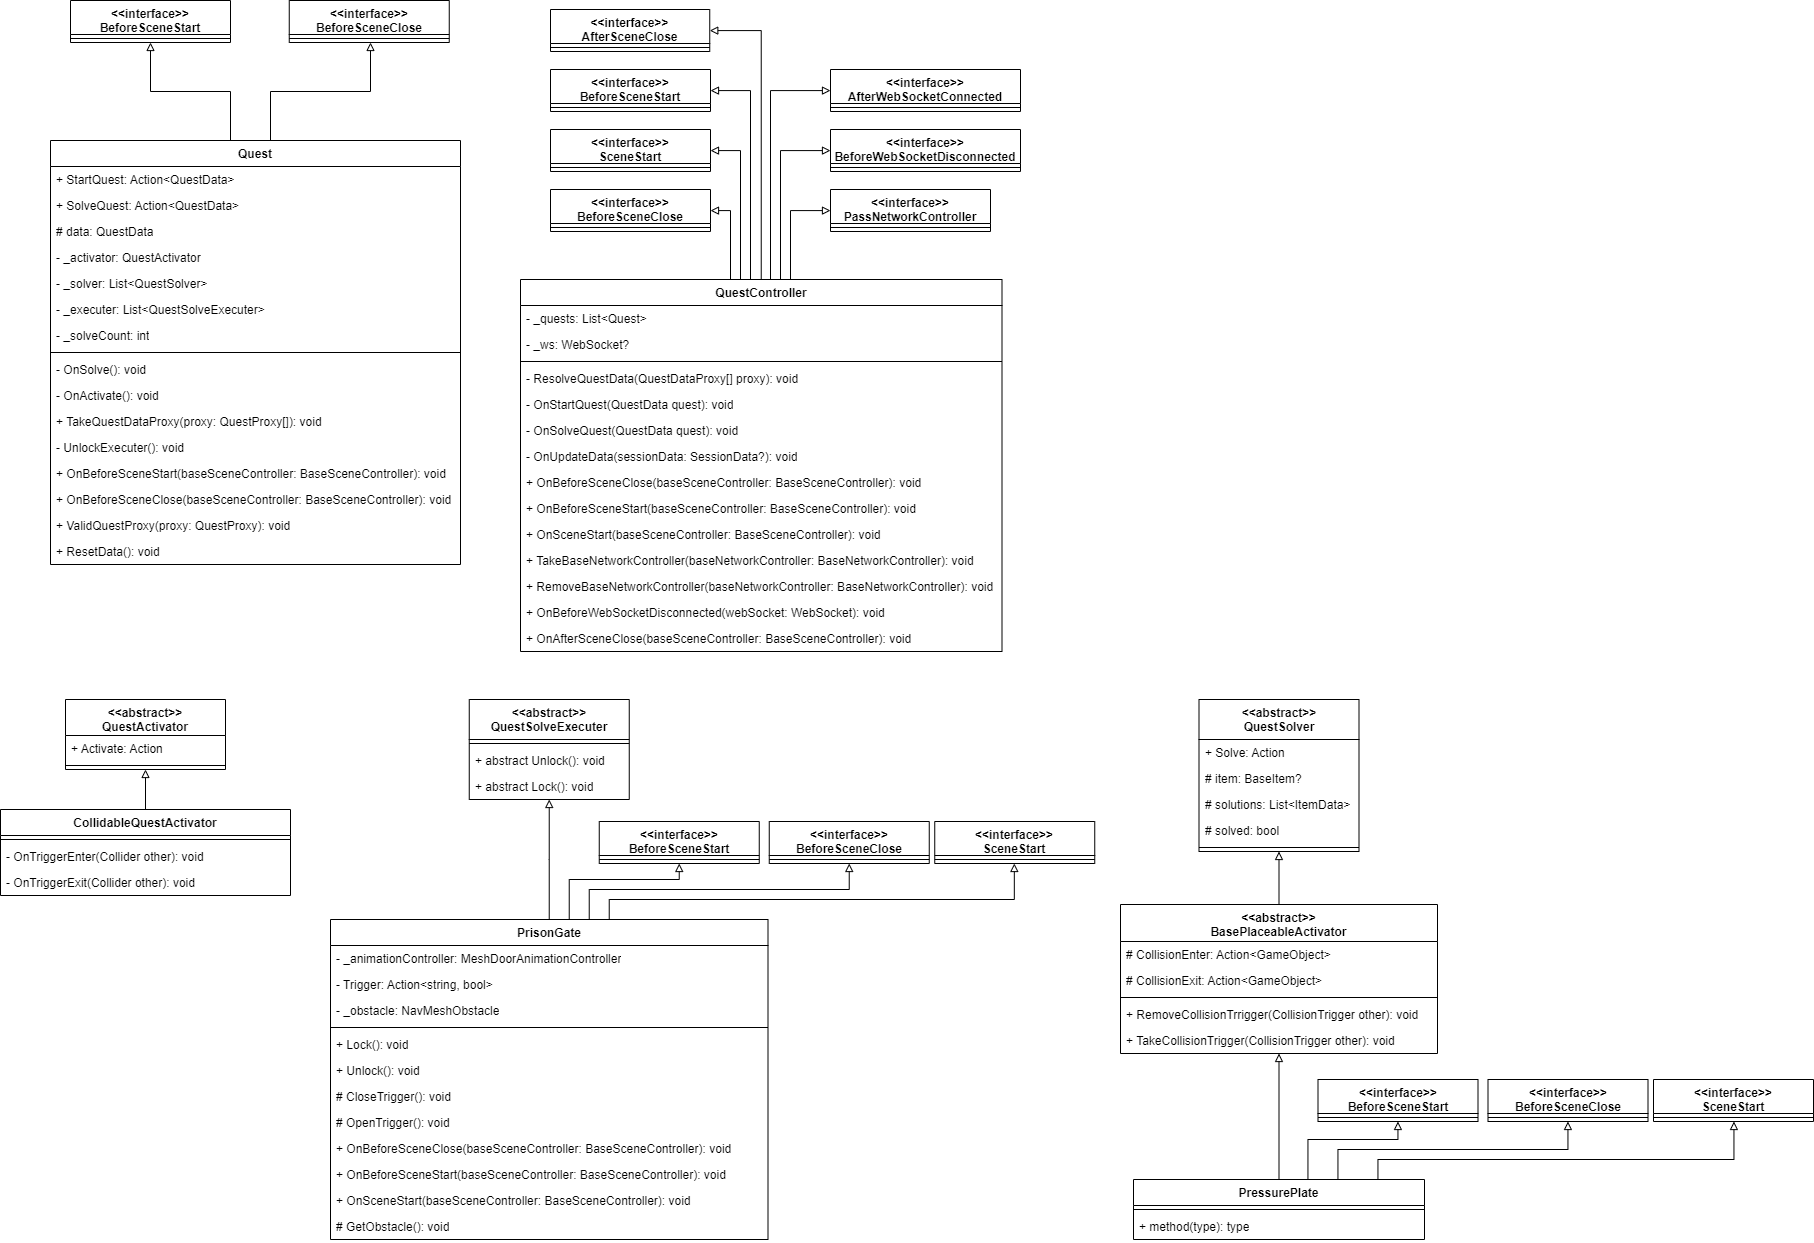
\includegraphics[width=1\linewidth]{content/pictures/QuestSystem.drawio.png}
\caption{UML-Diagramm zum Questsystem (Quelle: eigene Darstellung), (vollständig in Anhang \ref{sec:append_realisation_uml_quest})}
\label{fig:quest-system-uml}
\end{figure}

Abbildung \ref{fig:quest-system-uml} zeigt das entwickelte Questsystem, das zur strukturierten Einbettung von Rätsel in die Spielwelt dient. Die einzelnen Rätsel wurden in Anlehnung an \ac{RPG}-Spiele als Quests bezeichnet. Das System wurde modular konzipiert, sodass es sowohl in der Player- als auch in der Watcher-Anwendung integriert werden kann. Die folgenden Ausführungen gelten daher für beide Rollen gleichermaßen.

Zentrale Instanz des Systems ist der QuestController, der als überwachende Einheit fungiert. Er verwaltet Referenzen auf alle in der Szene existierenden Quests, empfängt Rückmeldungen über gelöste Quests vom Server und leitet diese an die entsprechenden Quests weiter. Gleichzeitig ist er für die Übermittlung neuer oder gelöster Quests an den Server verantwortlich. Wird bspw. eine Quest aktiviert, etwa durch das Freischalten eines neuen Raums, sorgt der QuestController dafür, dass diese zur Liste der aktiven bzw. gelösten Quests hinzugefügt wird.

Jede Quest selbst stellt eine einzelne Herausforderung dar und ist mit einer eindeutigen ID, einem Namen sowie einem Lösungsstatus ausgestattet. Sie überprüft selbstständig, ob sie gelöst wurde und informiert in diesem Fall den QuestController. Dazu besitzt sie Referenzen auf mehrere QuestSolver, also logische Einheiten, die eine Bedingung zur Lösung erfüllen müssen. Im Beispiel aus Abbildung \ref{fig:quest-system-uml} handelt es sich um eine Druckplatte mit Platzierungsfunktionalität, die dann aktiv wird, wenn ein passender Gegenstand korrekt platziert wurde. Sobald alle zugehörigen QuestSolver erfolgreich ausgelöst wurden, gilt die Quest als gelöst.

Vor der Lösung muss eine Quests jedoch zunächst aktiviert werden. Diese Funktion übernehmen sog. QuestActivator, auf die jede Quest ebenfalls Referenzen besitzt. Erst wenn alle Aktivatoren ausgelöst wurden, wird die Quest aktiv und kann gelöst werden. Im gezeigten Beispiel kommt ein CollidableQuestActivator zum Einsatz, der dann ausgelöst wird, wenn sich der Avatar des Players innerhalb eines definierten Colliders aufhält.

Sobald eine Quest erfolgreich abgeschlossen wurde, werden alle ihr zugewiesenen QuestSolveExecuter aktiviert. Diese Komponenten führen Aktionen aus, etwa das Öffnen einer Tür durch einen Animator (wie im Beispiel der Gefängnistür dargestellt).

\paragraph{Pathsystem}\label{sec:path-system}

Wie das Questsystem wurde auch das Pathsystem modular konzipiert, um eine Wiederverwendung sowohl in der Player- als auch in der Watcher-Anwendung zu ermöglichen. Dieses System ist insbesondere deshalb von zentraler Bedeutung, weil im Verlauf des Spiels neue Wege und Räume zugänglich gemacht werden, deren Freischaltung eng mit dem Fortschritt im Rätselsystem verknüpft sind.

\begin{figure}[ht]
\centering
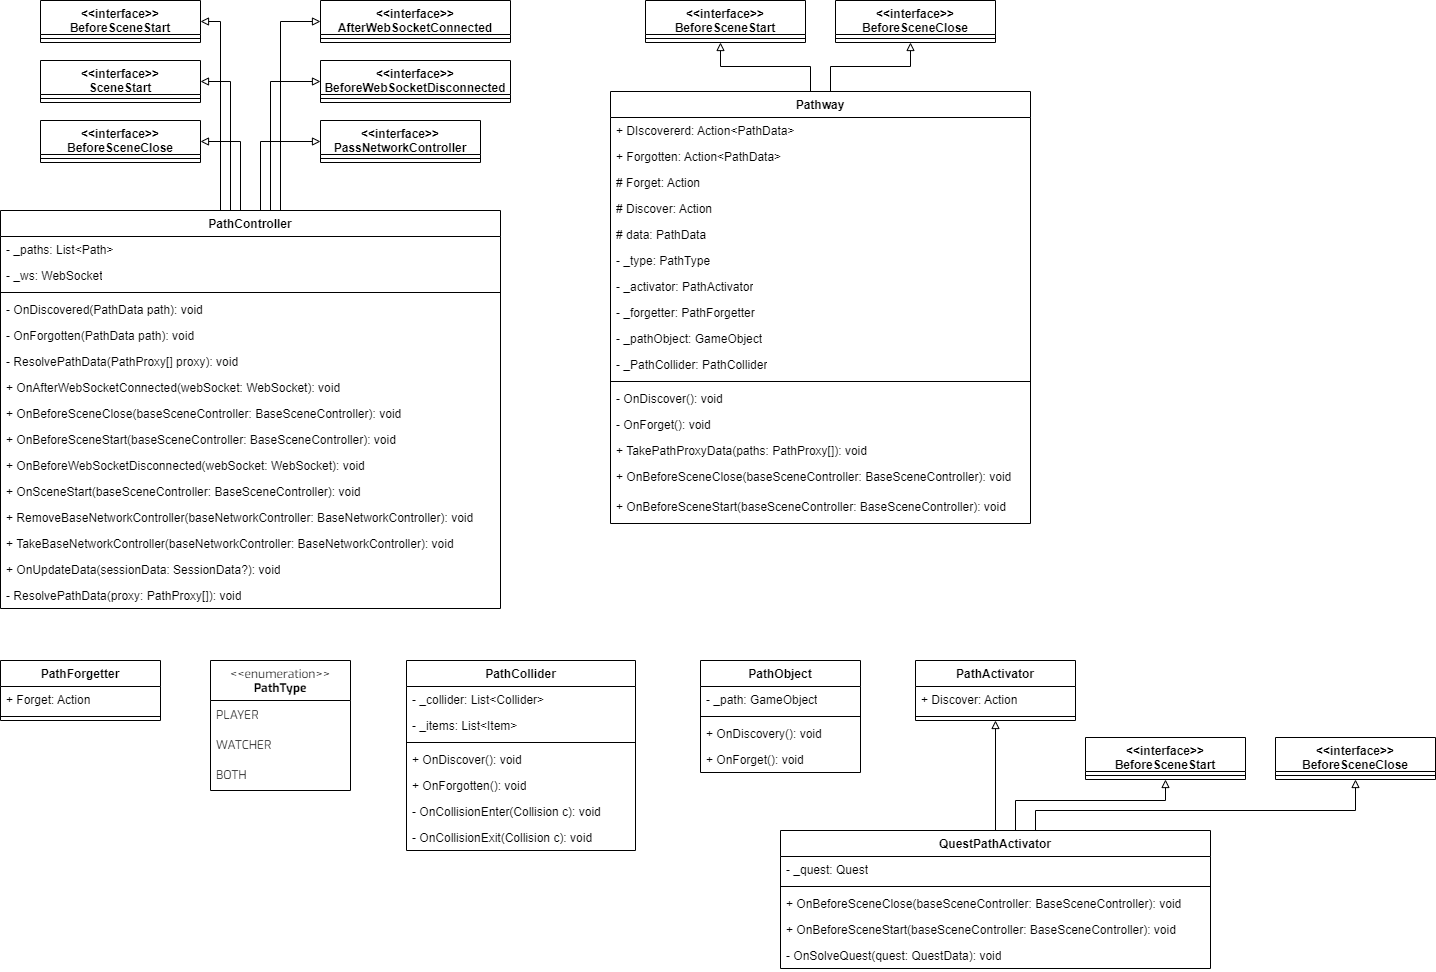
\includegraphics[width=1\linewidth]{content/pictures/PathSystem.drawio.png}
\caption{UML-Diagramm zum Pathsystem (Quelle: eigene Darstellung), (vollständig in Anhang \ref{sec:append_realisation_uml_path})}
\label{fig:path-system-uml}
\end{figure}

Abbildung \ref{fig:path-system-uml} zeigt das entworfene modulare Pathsystem, das in beiden Anwendungen eingebunden ist. Das zentrale Steuerelement stellt die Klasse PathController dar, welche, analog zum QuestController, für die Kommunikation mit dem Server verantwortlich ist. Sie empfängt und sendet Pathdaten und verwaltet sämtliche in der Spielszene konfigurierten Wege (Pathways).

Jeder Pathway verwaltet eine Reihe von Komponenten. Sog. PathActivator, die für die Freischaltung eines Weges zuständig sind und optional PathForgetter, welche bereits geöffnete Wege bei Bedarf wieder deaktivieren können. Darüber hinaus besitzt ein Pathway Referenzen auf die zugehörigen Objekte in der Spielwelt, ein sichtbares Wegobjekt (PathObject) sowie auf Kollisionsbereiche (PathCollider). Letztere spielen insbesondere bei der physischen Blockierung von noch nicht zugänglichen Bereichen eine Rolle.

Da im konzipierten Tutorial-Szenario keine bereits geöffneten Wege deaktiviert werden, wurde auf eine Implementierung konkreter PathForgetter verzichtet. Die Klasse QuestPathActivator aus dem in Abbildung \ref{fig:path-system-uml} dargestellten Beispiel übernimmt die Aufgabe, nach dem erfolgreichen Abschluss einer bestimmten Quest den zugehörigen Pathway zu aktivieren.

Wird ein Pathway aktiviert, so wird das entsprechende \ac{3D}-Objekt (PathObject) in der Szene sichtbar geschaltet und die zugehörigen PathCollider deaktiviert, sodass der neue Bereich für den Player zugänglich wird. Auf die genaue Funktionsweise der PathCollider und deren Bedeutung im Gesamtsystem wird im späteren Kapitel \ref{sec:difficulties-placement} detailliert eingegangen.

\paragraph{User-Interfaces}

\begin{figure}[ht]
\centering
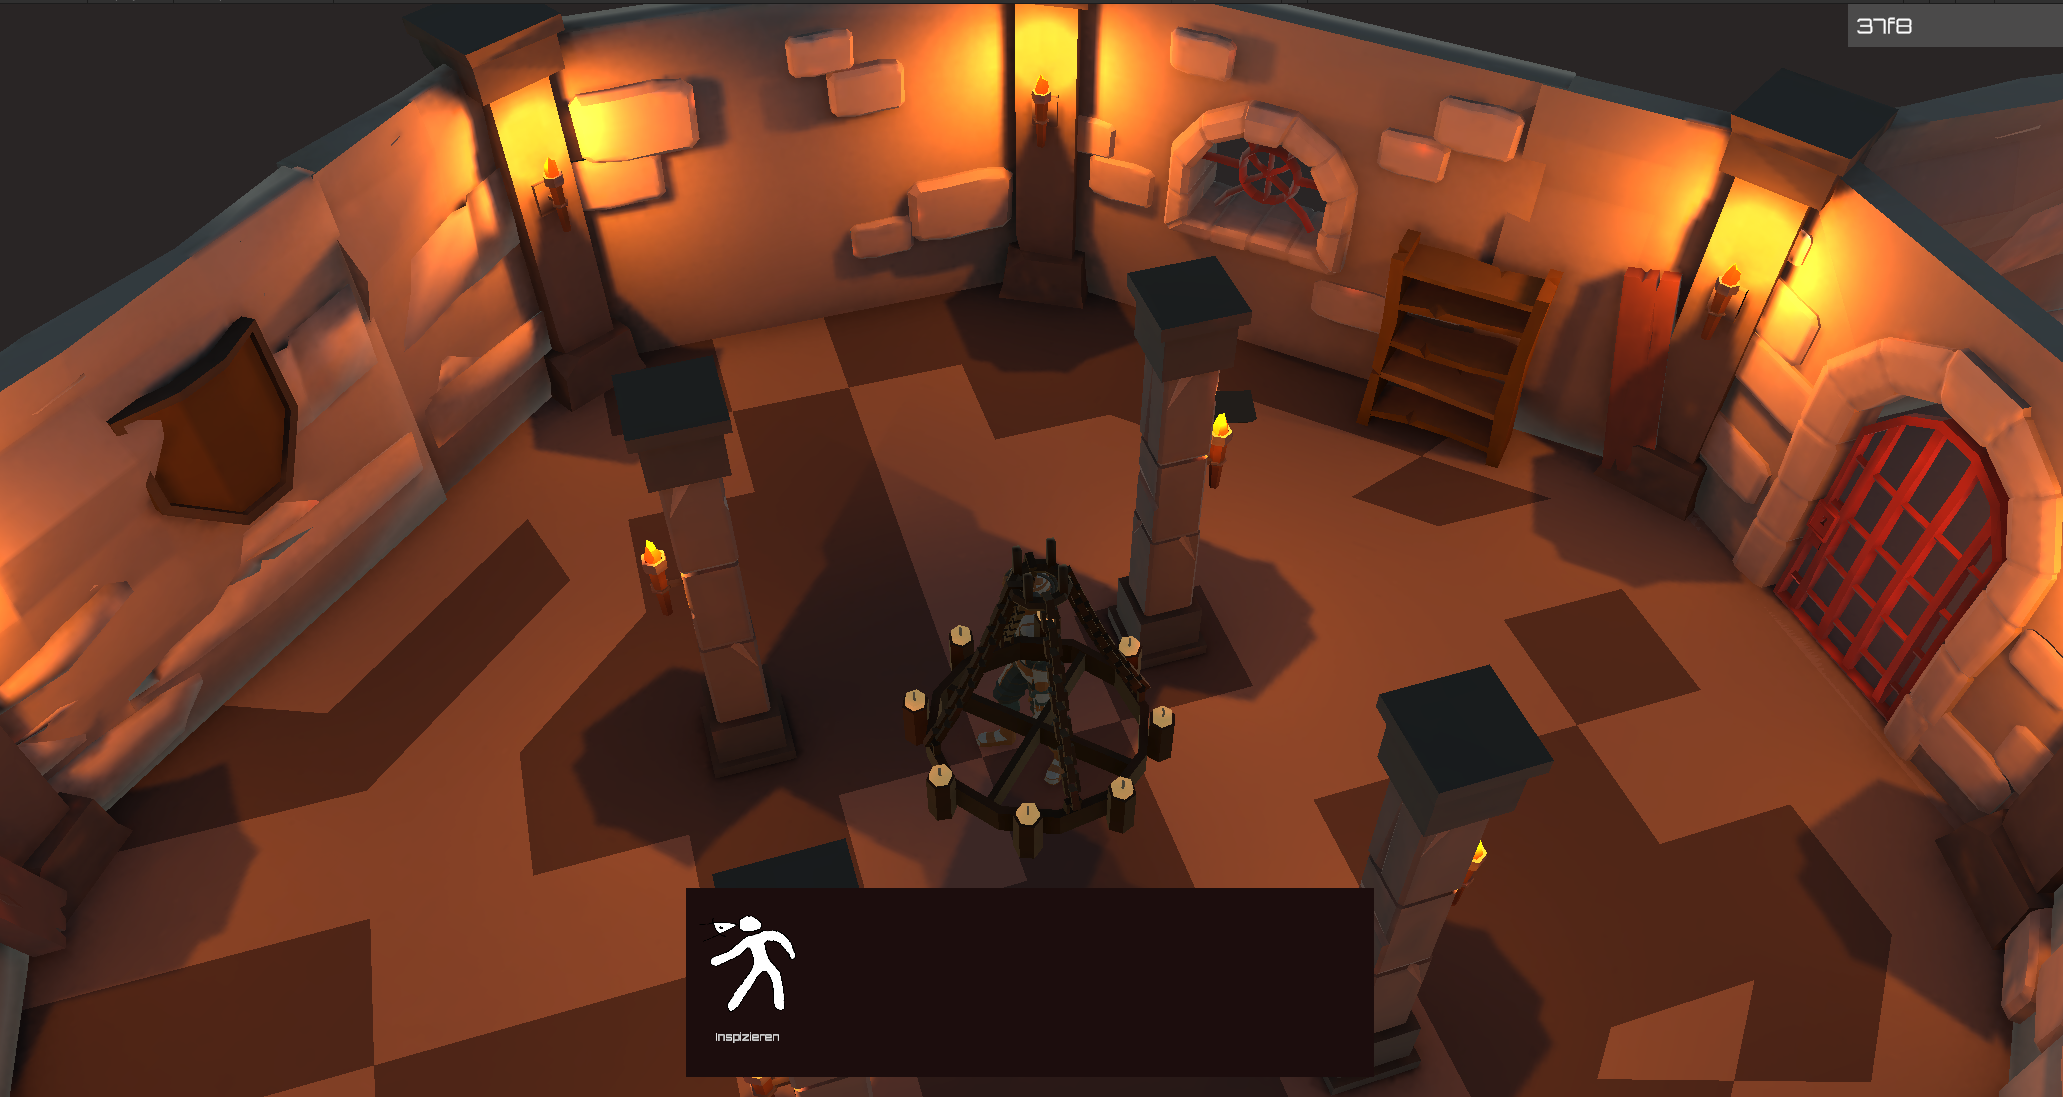
\includegraphics[width=1\linewidth]{content/pictures/UI.PNG}
\caption{UI des Players (Quelle: eigene Darstellung)}
\label{fig:player-ui}
\end{figure}

Abbildung \ref{fig:player-ui} zeigt die Ansicht, die der Player in der Spielwelt hat. Unten in der Mitte wird die Interaktionsleiste angezeigt, über welche der Player Interaktionen mit der Spielwelt ausführen kann. Anhand des gezeigten Bildes kann er derzeit nur in die First-Person-Sicht wechseln. Sobald er an einen interaktiven Gegenstand kommt, erscheint in der Leiste seine entsprechenden Interaktionsfunktionen. Dieses Konzept ist an Spiele wie \say{Diablo 4} oder \say{Baldurs Gate 3} angelehnt, bei denen über eine ähnliche Aktionsleiste Fähigkeiten und Angriffe ausgeführt werden können  (vgl. \citealp{blizzard_entertainment_diablo_2023,larian_studios_baldurs_2023}).

\subsection{Watcher-Anwendung}

Die Watcher-Anwendung stellt, ebenso wie die Player-Anwendung, eine der beiden \say{Views} innerhalb der umgesetzten \ac{MVC}-Architektur dar. Sie umfasst die grundlegende Spielwelt aus der Perspektive des Watchers und bildet zugleich die Grundlage für dessen Interaktionsmöglichkeiten mit der Umgebung.

Analog zur Player-Anwendung basiert auch die visuelle Darstellung in der Watcher-Anwendung auf den Basisobjekten der Spielwelt, die mittels sog. Prefab Variants darstellungsspezifisch angepasst wurden. Auf diese Weise wird eine konsistente Gestaltung der Umgebung sichergestellt, wobei sich für die jeweilige Perspektive relevanten Unterschiede manifestieren.

Ein wesentlicher Unterschied zur Player.Anwendung besteht in der Existenz zweier unterschiedlicher Betriebsmodi. Der Watcher kann entweder mittels einer \ac{AR}-Integration oder über eine \ac{3D}-Ansicht auf die Spielwelt zugreifen. Während die \ac{AR}-Variante für den späteren produktiven Einsatz konzipiert ist, wurde die \ac{3D}-Integration primär für Entwicklungs- und Testzwecke realisiert. Sie ermöglicht, den aktuellen Entwicklungsstand direkt im Unity-Editor zu überprüfen, ohne dass die Anwendung jeweils auf ein Smartphone übertragen und oder ausgeführt werden muss.

\paragraph{Steuerung der Anwendung}

Wie bereits in der Player-Anwendung spielt auch in der Watcher-Anwendung die Kamerasteuerung eine zentrale Rolle. Allerdings muss sie hier differenzierter betrachtet werden, da sich die Anforderungen in den beiden Modi, \ac{AR} und \ac{3D}, deutlich unterscheiden.

In der \ac{AR}-Variante übernimmt das Endgerät die Kamerasteuerung automatisch über die Sensorsysteme. Eine manuelle Steuerung den Watcher ist daher nicht erforderlich. Für die Interaktion mir der Anwendung genügt eine einfache Single-Touch-Eingabe, etwa zur Platzierung von Gegenständen. Wie \cite{reinhard_augmented_2022} zeigt, sind solche minimalistischen Eingabekonzepte typisch für \ac{AR}-Anwendungen auf Mobilgeräten (vgl. \citealp[S. 66ff]{reinhard_augmented_2022}).

 Im Gegensatz dazu erfordert die \ac{3D}-Variante der Anwendung eine explizite Kamerasteuerung, ähnlich wie in der Player-Anwendung. In diesem Kontext sind zunächst grundsätzliche Überlegungen zum zugrunde liegenden Kamerakonzept notwendig. Mobile Spiele nutzen unterschiedliche Steuerungsarten. Einige verzichten gänzlich auf eine freie Kamerabewegung, andere folgen einem Spieler-Avatar, während wieder andere eine vollständige Kontrolle über die Kamera ermöglichen.

 Für die \ac{3D}-Variante wurde bewusst auf die Implementierung eines Joystick-basierten \ac{HUD}-Overlays verzichtet, da dieses der intuitiven Touchsteuerung-Nutzung widerspricht und Interaktionsmöglichkeiten unnötig einschränkt. Stattdessen orientierte sich die Umsetzung an Spielen, die auf Touch-Gesten basieren, etwa \say{Die Sims Mobile} oder \say{Outlanders} (vgl. \citealp{arts_sims_2018, pomelo_games_outlanders_2019}). Diese nutzen ein Kamerasystem, wie es aus klassischen Strategiespielen, etwa wie der \say{Anno}-Reihe, bekannt ist, eine, sog. \ac{RTS}-Kamera, bei der ein unsichtbares LookAt und Follow Objekt durch Nutzereingaben verschoben wird, dem die Kamera folgt (vgl. \citealp{ubisoft_mainz_ubisoft_2019}). 

Auch in der Watcher-Anwendung wurde dieser \ac{RTS}-Ansatz umgesetzt. Dabei wird die Kamera durch folgende Touch-Gesten gesteuert.
Der Single-Touch für das Platzieren und Entfernen von Gegenständen in der Spielwelt, die Yaw-Geste für die horizontale Rotation der Kameraansicht zur Veränderung der Blickrichtung, die Zoom-Geste für die Annäherung und Entfernung zur Spielwelt und die Pan-Geste zur Bewegung der Kamera innerhalb der Spielwelt.

Die Pitch-Geste wurde bislang nicht implementiert, da für sie in der aktuellen Fassung der Anwendung kein konkreter Anwendungsfall identifiziert wurde.

\paragraph{Aufbau des Nutzerflows}

Da die Hauptaufgabe des Watchers im Verwalten und Platzieren von Gegenständen besteht, musste zunächst ein geeigneter Nutzerfluss entwickelt werden, der den spezifischen Anforderungen der Anwendung gerecht wird. 

Als Referenz dient hierbei das Spiel \say{Outlanders}, dessen Spielaufbau und Menünavigation zentrale Parallelen zur Watcher-Anwendung aufweist (vgl. \citealp{pomelo_games_outlanders_2019}). In Outlanders übernimmt der Spieler die Rolle eines Anführers, der eine Siedlung errichten muss. Der Zugriff auf entsprechende Bau- und Verwaltungsfunktionen erfolgt dabei über ein zentrales Hauptmenü, das in die Menüleiste des Spiels integriert ist. Dieses Interface-Prinzip wurde aufgegriffen, da es dem Watcher ermöglicht, sich zunächst frei in der Spielwelt zu bewegen, sei es durch die \ac{AR}-Kamera oder das \ac{RTS}-Kamerasystem, um anschließend über ein übersichtliches Menü Gegenstände zu platzieren oder dem Player zu senden.

\begin{figure}[ht]
\centering
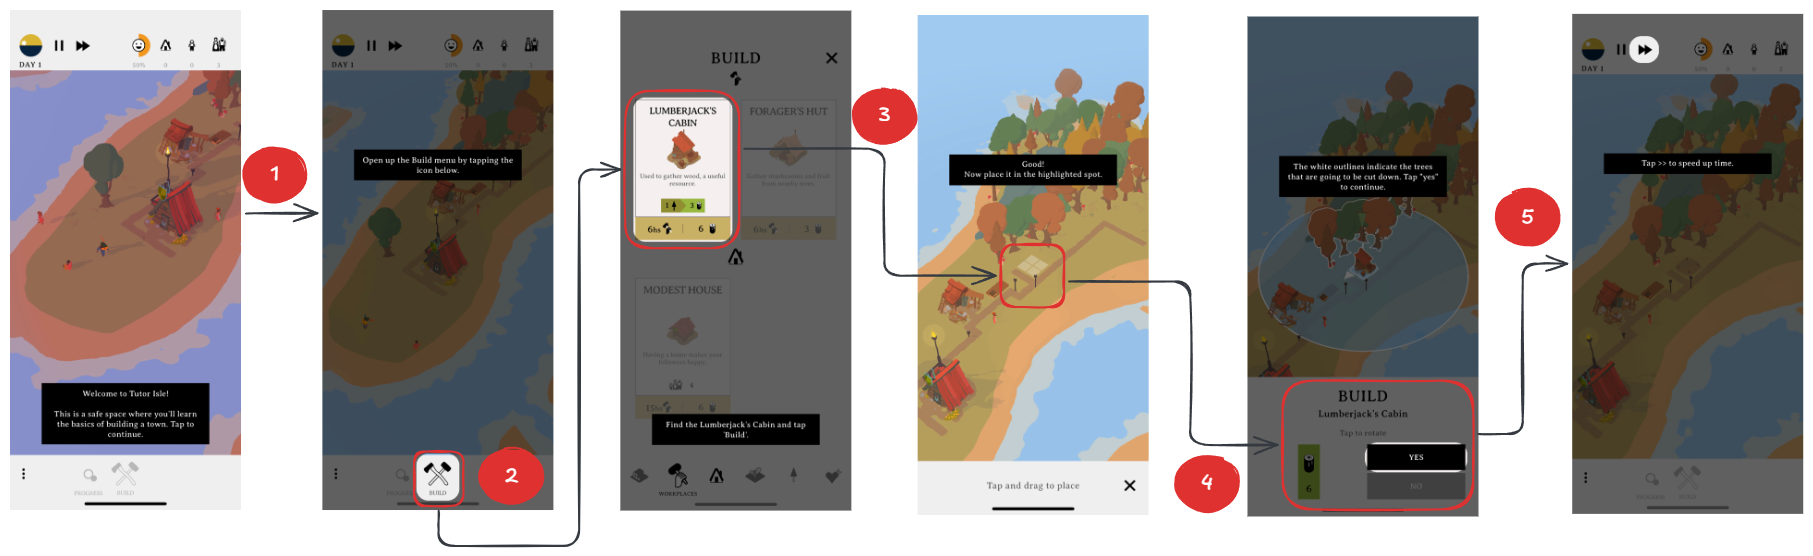
\includegraphics[width=1\linewidth]{content/pictures/Nutzerflow.png}
\caption{Nutzerfluss beim Gebäudebau in Outlanders (Screenshots von \cite{coates_game_nodate}), (Quelle: eigene Darstellung)}
\label{fig:userflow-outlanders-build}
\end{figure}

Zu Beginn kann sich der Spieler frei durch die Spielwelt bewegen (1). Möchte er ein Gebäude für seine Bevölkerung errichten, so wählt er über die Menüleiste am unteren Bildschirmrand den Reiter \say{Build} aus (2). Daraufhin öffnet sich ein Overlay-Menü, das als Baumenü fungiert. Innerhalb dieses Menüs kann der Spieler zwischen verschiedenen Kategorien von Gebäuden und anderen Bauelementen wählen. Nach der Auswahl eines gewünschten Gebäudes schließt sich das Menü automatisch und der Spieler muss eine Position in der Spielwelt auswählen, an der das gewählte Gebäude platziert werden soll (3). Sobald eine Platzierung ausgewählt wurde, erscheint ein weiteres, halbseitiges Bestätigungsmenü. Erst nach der Bestätigung durch den Spieler wird das Gebäude an der gewünschten Stelle errichtet (4). Anschließend wird das Bestätigungsmenü geschlossen und die freie Navigation durch die Spielwelt ist erneut möglich (5).

Sowohl der strukturierte Nutzerfluss dieses Baumenüs als auch die visuelle Gestaltung des Interface-Designs hatten einen prägenden Einfluss auf die ersten Benutzeroberflächen der Watcher-Anwendung.

\begin{figure}[ht]
\centering
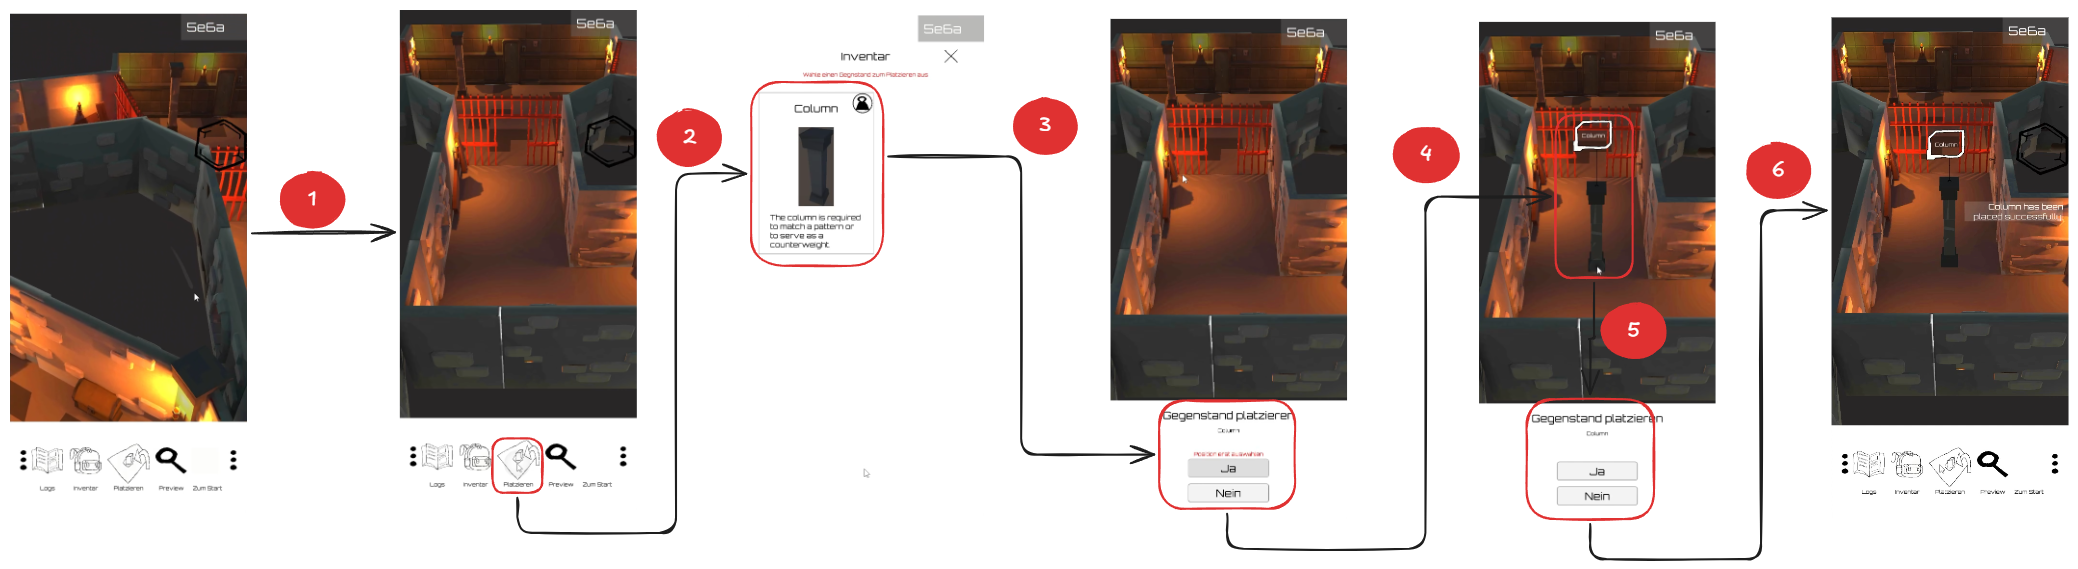
\includegraphics[width=1\linewidth]{content/pictures/PlacementFlow.png}
\caption{Nutzerfluss des Platzierens eines Gegenstandes (Quelle: eigene Darstellung)}
\label{fig:userflow-placement-cm}
\end{figure}

Abbildung \ref{fig:userflow-placement-cm} visualisiert den Nutzerfluss, den der Watcher durchläuft, um einen Gegenstand in der Spielwelt zu platzieren. Dieser Ablauf orientiert sich stark am zuvor beschriebenen Platzierungsprozess aus Outlanders.

Zunächst kann sich der Watcher frei durch die Spielwelt bewegen (1). Möchte er nun an einer bestimmten Stelle einen Gegenstand platzieren, öffnet er über das \say{Platzieren}-Menü das Platzierungsmenü, woraufhin sich ein Overlay-Menü einblendet (2). Innerhalb dieses Menüs wählt er einen konkreten Gegenstand aus. Nach der Auswahl erscheint ein weiteres Menü, das einen kleinen Bereich des Bildschirms überlagert und den Watcher zur Auswahl einer geeigneten Platzierungsposition auffordert (3). Sobald eine Position gewählt wurde, wird dem Nutzer an dieser Stelle eine Vorschau des zu platzierenden Gegenstands angezeigt (4). Über das weiterhin geöffnete Menü kann die Auswahl nun bestätigt werden (5). Nach der Bestätigung wird der Gegenstand an der gewählten Position dauerhaft in der Spielwelt platziert (6).

\begin{figure}[ht]
\centering
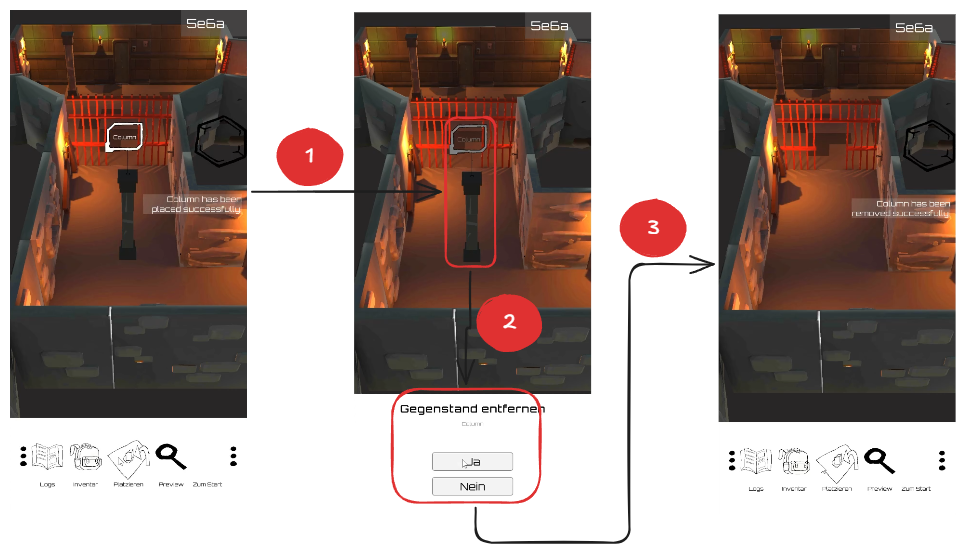
\includegraphics[width=1\linewidth]{content/pictures/RemovePlacementFlow.png}
\caption{Nutzerfluss des Entfernens eines Gegenstandes (Quelle: eigene Darstellung)}
\label{fig:userflow-removement-cm}
\end{figure}

Abbildung \ref{fig:userflow-removement-cm} zeigt den Nutzerfluss, den ein Watcher durchläuft, wenn er einen zuvor platzierten Gegenstand wieder entfernen möchte. Zu Beginn kann sich der Watcher frei durch die Spielwelt bewegen. Sobald jedoch ein Gegenstand entfernt werden soll, um ihn an einer anderen Position neu zu platzieren, wählt der Watcher das entsprechende Gegenstands-Objekt durch einen Touch in der Spielwelt aus (1). Das Tooltip des ausgewählten Gegenstands verändert daraufhin seine Farbe, um die Auswahl visuell hervorzuheben. Gleichzeitig öffnet sich am unteren Bildschirmrand ein kleines Menü, über das die Entfernung des Gegenstands bestätigt werden kann (2). Nach der Bestätigung wird das Objekt aus der Spielwelt entfernt, und der Watcher kann sich erneut frei durch die Umgebung bewegen (3).

\begin{figure}[ht]
\centering
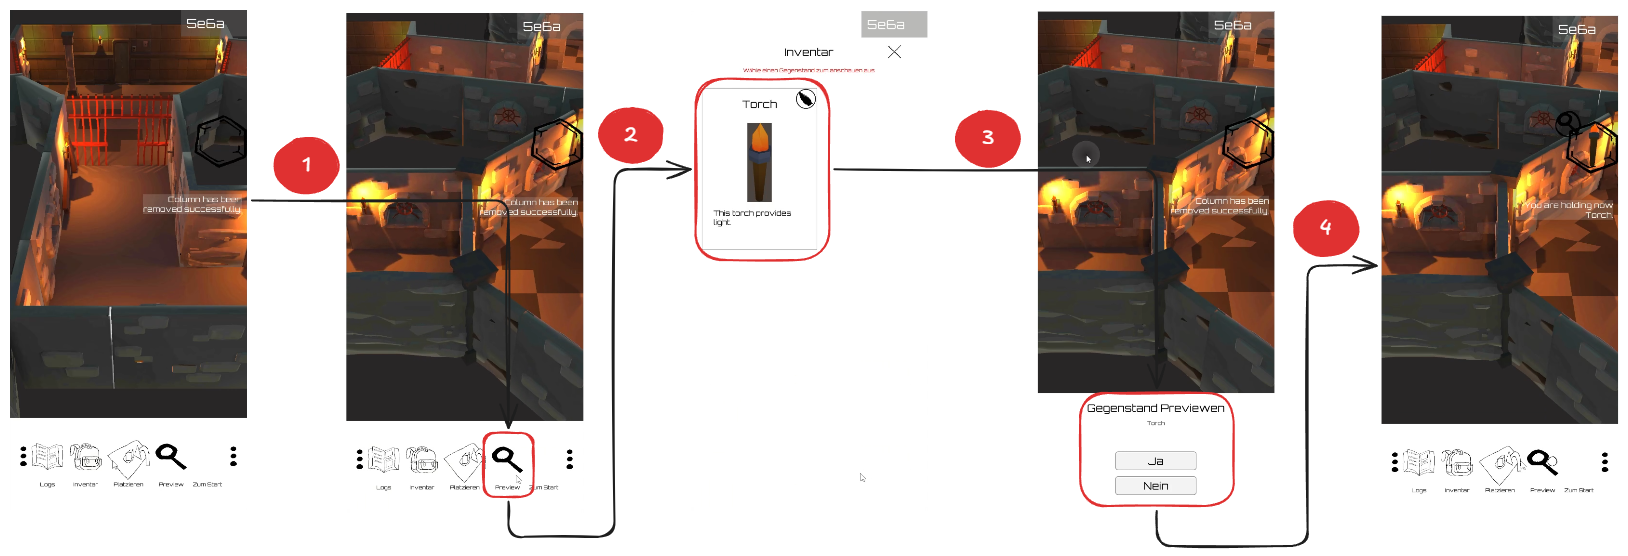
\includegraphics[width=1\linewidth]{content/pictures/PreviewFlow.png}
\caption{Nutzerfluss des Previewen eines Gegenstandes (Quelle: eigene Darstellung)}
\label{fig:userflow-preview-cm}
\end{figure}

Neben dem Platzieren von Gegenständen stellt das Übermitteln (Previewen) eines Gegenstrandes an den Player eine weitere zentrale Funktion des Watchers dar. Der bereits etablierte Nutzerfluss, der sich am Beispiel Outlanders orientiert und erfolgreich für das Platzieren von Gegenständen adaptiert wurde, dient ebenfalls als Grundlage für die Gestaltung des Preview- Sendeprozesses (vgl. Abbildung \ref{fig:userflow-preview-cm}).

Zunächst kann sich der Watcher frei durch die Spielwelt bewegen. Um einen Gegenstand den an den Player zu senden, öffnet er das \say{Preview}-Menü, das rechts neben dem \say{Platzieren}-Menü positioniert ist (1). Durch das Anklicken dieses Menüs wird eine Galerie geöffnet, die den gesamten Bildschirm einnimmt. Innerhalb dieser Galerie kann der Watcher einen Gegenstand aus einer Auswahl wählen (2). Nach der Auswahl erscheint ein Bestätigungsmenü, über das die Entscheidung final bestätigt werden muss (3). Nach erfolgreicher Bestätigung wird das Bestätigungsmenü geschlossen und der Watcher kann sich im freien Navigationsmodus bewegen. In der rechten, halbhohen Bildschirmhälfte wird nun visuell angezeigt, welchen Gegenstand der Player aktuell mit sich führt (4).

\begin{figure}[ht]
\centering
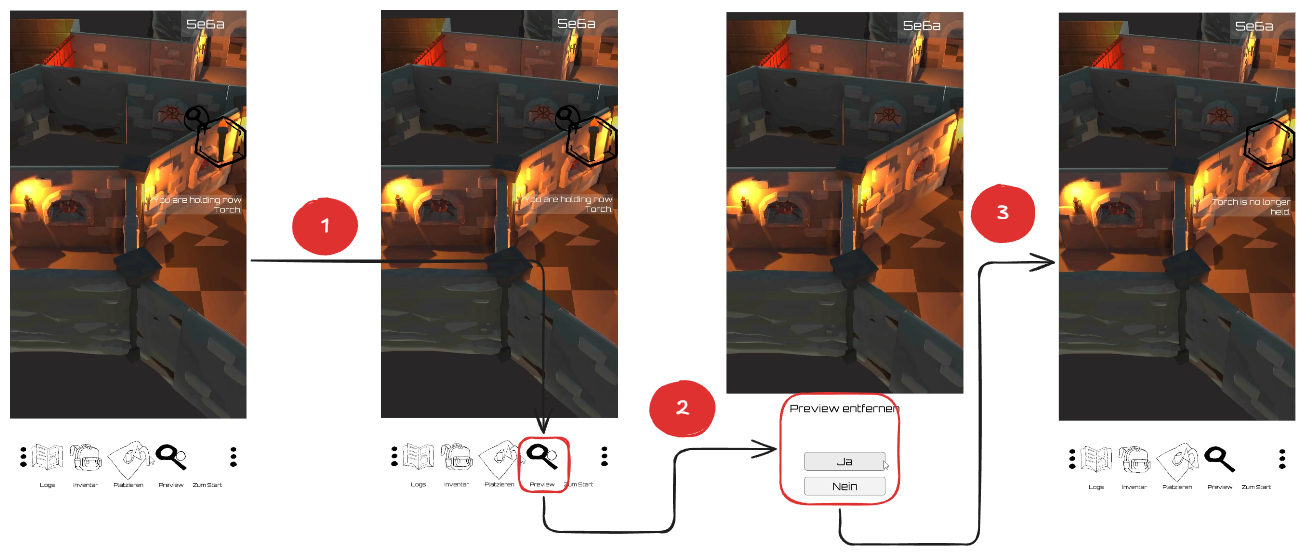
\includegraphics[width=1\linewidth]{content/pictures/RemovePreviewFlow.png}
\caption{Nutzerfluss des Entfernens der Preview eines Gegenstandes (Quelle: eigene Darstellung)}
\label{fig:userflow-remove-preview-cm}
\end{figure}

Abbildung \ref{fig:userflow-remove-preview-cm} veranschaulicht den Nutzerfluss für das Entfernen eines des Players gepreviewten Gegenstands. Ausgangspunkt ist erneut der freie Navigationsmodus, in dem sich der Watcher innerhalb der Spielwelt bewegen kann. Sobald er einen Hinweis erhält, dass ein zuvor übermittelter Gegenstand wieder entfernt werden soll, öffnet er, analog zum Previewprozess, das \say{Preview}-Menü (1). Anders als beim erstmaligen Previewen eines Gegenstandes öffnet sich jedoch nicht die vollständige Galerieansicht, sondern unmittelbar ein Bestätigungsdialog, der abfragt, ob der aktuell vom Player getragene Gegenstand entfernt werden soll (2). Wird diese Abfrage bestätigt, wird der Gegenstand entfernt und der Watcher kehrt in den freien Navigationsmodus zurück. Zusätzlich verschwindet die entsprechende Visualisierung des Gegenstands aus der rechten, halbhohen Bildschirmanzeige (3). 

\subsection{Server-Anwendung}

Die Server-Anwendung bildet, wie bereits in der Einleitung dieses Kapitel erläutert, das zentrale Element innerhalb der \ac{MVC}-Architektur. Dabei stellt sich die grundlegende Frage, auf welche Weise und Einsatz weicher Netzwerkprotokolle die Kommunikation zwischen den einzelnen Anwendungskomponenten realisiert wird.

Zunächst gilt es, die Art des Servers zu bestimmen. Aus dem Aufbau der \ac{MVC}-Architektur geht hervor, dass die View-Komponente vom Model sowie vom Controller entkoppelt ist. Daraus ergibt sich die Notwendigkeit, ein eigenständiges System für den Server zu implementieren das als zentrale Kommunikationsschnittstelle für die verschiedenen View-Instanzen fungiert. Auf Basis der in den Grundlagen zur Netzwerkinfrastruktur vorgestellten Konzepte lassen sich im Hinblick auf spezifische Anforderungen der Architektur verschiedene Ansätze systematisch eingrenzen und bewerten.

\paragraph{Bestimmung der Netzwerk-Topologie}

Eine klassische \\ Client-Server-Netzwerkinfrastruktur kann für den vorliegenden Anwendungsfall ausgeschlossen werden, da weder der Server noch ein dedizierter Client die vollständige Simulation der Spielwelt übernehmen soll. Stattdessen verwalten die einzelnen View-Komponenten ihre jeweilige Spielweltinstanz autonom und übermitteln lediglich Veränderungen relevanter Kerndatenelemente an den Server.

Auch ein \ac{P2P}-Modell erweist sich als ungeeignet, da hierfür sämtliche Anwendungen direkt miteinander verbunden sein müssten. Dies würde zu einem hochgradig komplexen Kommunikationsnetz führen, in dem jeder Client kontinuierlich Spielzustände mit allen anderen Clients synchronisieren müsste. Ein Aufwand, der insbesondere bei wachsender Anzahl an Teilnehmern schnell an Skallierungsgrenzen stößt und somit nicht mehr zuverlässig realisierbar wäre.

Verbleibende geeignete Architekturen sind das Modell der \say{Distributed Authorities} sowie des sog. Relay-System. Letzteres ermöglicht eine serververmittelte Kommunikation zwischen den Anwendungen, ohne dass ein dedizierter Spielserver die zentrale Spiellogik simulieren muss. Der Server fungiert in diesem Fall lediglich als Relaisinstanz zur Weiterleitung der Nachrichten. Im Modell der Distributed Authorities hingegen ist jeder verbundene Client für die lokale Simulation der Spielwelt verantwortlich und übermittelt relevante Zustandsänderungen an einen zentralen Service, der eine globale Konsistenz des Spielzustands gewährleistet, indem er die Informationen an alle übrigen Clients verteilt.

Die Kombination beider Ansätze stellt für die Anwendung von Connecting-Minds die geeignete Architektur dar, da sie eine dezentrale Verwaltung der Spielwelt mit einer effizienten und skalierbaren Kommunikationsstruktur verbindet.

\paragraph{Bestimmung der Kommunikationsprotokolle}

\begin{figure}[ht]
\centering
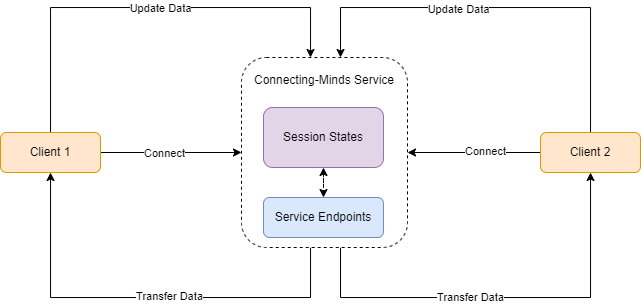
\includegraphics[width=1\linewidth]{content/pictures/CM-Archticture.png}
\caption{Connecting-Minds Infrastruktur (Quelle: eigene Darstellung)}
\label{fig:cm-topology}
\end{figure}

Nachdem eine geeignete Netzwerk-Topologie bestimmt wurde (vgl. Abbildung \ref{fig:cm-topology}), ist im nächsten Schritt festzulegen, auf welche Weise die Anwendungen im Detail miteinander kommunizieren sollen. Zur Einordnung der Kommunikationsprozesse dient das \ac{OSI}-Modell, das die Netzwerkkommunikation in sieben funktionale Schichten unterteilt vgl. \citealp{a1_osi-modell_2025}).

Für die Kommunikation zwischen verteilten Anwendungen ist insbesondere die Transportschicht (Layer 4) von zentraler Bedeutung. Jeglicher Datenaustausch auf Anwendungsebene muss diese Schicht durchlaufen, da sie für den zuverlässigen Transport von Datenpaketen zwischen Endgeräten verantwortlich ist. Innerhalb der Transportschicht kommen hauptsächlich zwei Protokolle zum Einsatz: Das \ac{TCP} sowie das \ac{UDP} (vgl. \citealp{talkb1nary_transport_nodate}). Beide Protokolle unterscheiden sich grundlegend hinsichtlich ihrer Zuverlässigkeit, Latenz und Kommunikationsweise und stellen somit unterschiedliche Vor- und Nachteile für die Anforderungen der Spielarchitektur dar.

\begin{figure}[ht]
\centering
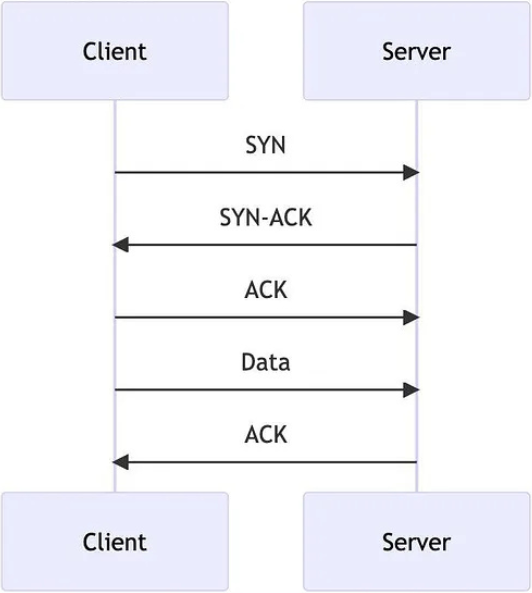
\includegraphics[width=0.5\linewidth]{content/pictures/TCP-Network.png}
\caption{Kommunikationsverbindung über TCP (Quelle: \citealp{mygames_unity_2024})}
\label{fig:tcp}
\end{figure}

Das \ac{TCP} ist ein verbindungsorientiertes Protokoll, das vor dem eigentlichen Datenaustausch eine stabile Verbindung zwischen Sender und Empfänger aufbaut. Diese Verbindung gewährleistet eine zuverlässige Übertragung, bei der sämtliche Datenpakete vollständig und in der korrekten Reihenfolge beim Empfänger eintreffen. Der sog. Drei-wege-Handshake, der diesen Verbindungsaufbau ermöglicht, ist in Abbildung \ref{fig:tcp} dargestellt. Zunächst erzeugen sowohl der Client als auch der Server jeweils einen Socket für die Kommunikation über \ac{TCP}. Anschließend sendet der Client ein \ac{SYN}-Segment an den Server, in dem der gewünschte Zielport spezifiziert ist. Der Server akzeptiert dieses \ac{SYN}-Segment, generiert seinerseits einen Socket und antwortet mit einem \ac{SYN}-\ac{ACK}-Segment. Der Client bestätigt dies durch ein \ac{ACK}-Segment, wodurch eine bidirektionale Verbindung hergestellt wird (vgl. \citealp{mygames_unity_2024}).

Im Gegensatz dazu ist das \ac{UDP} verbindungslos und damit wesentlich einfacher aufgebaut als das \ac{TCP}. Es initiiert keinen Verbindungsaufbau, sondern versendet Datenpakete direkt an den Empfänger, ohne die Garantie, dass diese tatsächlich ankommen oder in der richtigen Reihenfolge eintreffen. Aufgrund dieser Eigenschaft weist das \ac{UDP} eine deutlich geringere Latenz auf und eignet sich insbesondere für Anwendungen mit hoher Echtzeitanforderung wie etwa Online-Multiplayer-Spiele. Abbildung \ref{fig:udp} visualisiert das Prinzip der \ac{UDP}-Kommunikation. Der Verzicht auf Mechanismen zur Sicherstellung der Zustellung erfordert jedoch eine besonders sorgfältige Implementierung und Fehlerbehandlung auf Anwendungsebene (vgl. \citealp{mygames_unity_2024}).

\begin{figure}[ht]
\centering
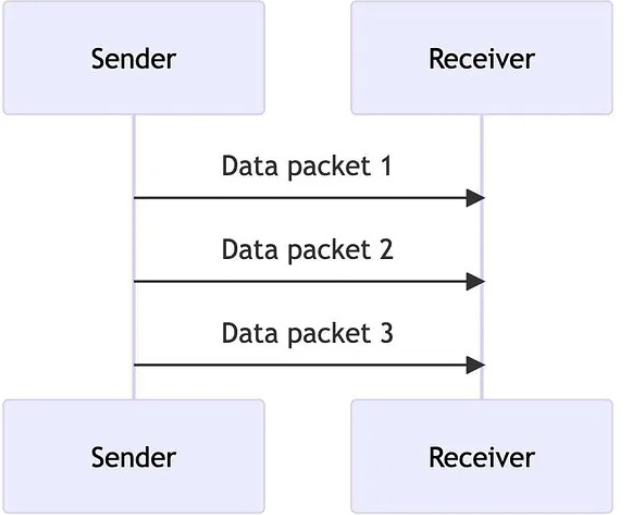
\includegraphics[width=0.5\linewidth]{content/pictures/UDP-Network.png}
\caption{Kommunikation über UDP (Quelle: \citealp{mygames_unity_2024})}
\label{fig:udp}
\end{figure}

Auf Grundlage der Basisprotokolle \ac{TCP} und \ac{UDP} existieren verschiedene Erweiterungen, die spezifische Anforderungen an die Netzwerkkommunikation adressieren. Eine davon ist das WebSocket-Protokoll, ein Anwendungsprotokoll (Application Layer Protocol), das auf das \ac{TCP} aufsetzt. WebSockets ermöglichen die Etablierung einer dauerhaften, bidirektionalen Kommunikationsverbindung zwischen zwei Teilnehmern, typischerweise zwischen einem Webbrowser und einem Server. Im Gegensatz zum klassischen \ac{HTTP}, das nach dem Request-Response-Prinzip funktioniert, erlaubt WebSocket eine kontinuierliche, ereignisgetriebene Kommunikation. Dadurch kann der Server proaktiv Nachrichten an den Client übermitteln, ohne das dieser zuvor eine Anfrage senden muss (vgl. \citealp{mygames_unity_2024}).

\begin{figure}[ht]
\centering
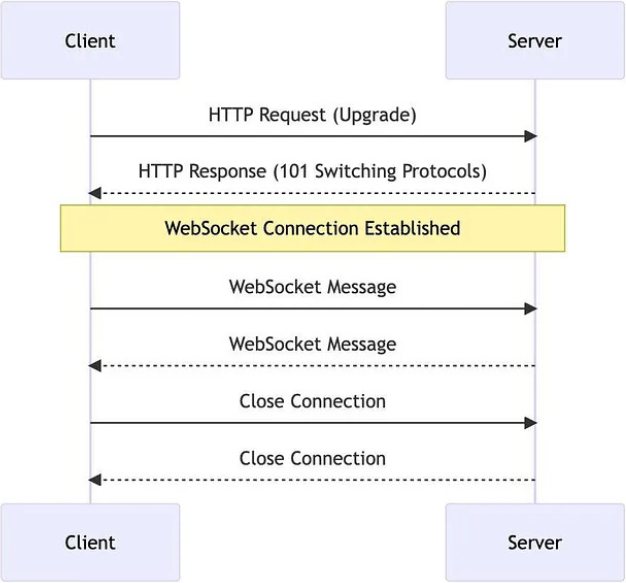
\includegraphics[width=0.5\linewidth]{content/pictures/WebSocket-Network.png}
\caption{Kommunikation über WebSocket (Quelle: \citealp{mygames_unity_2024})}
\label{fig:ws}
\end{figure}

Für die gewählte Netzwerkarchitektur erweist sich das WebSocket-Protokoll als besonders geeignet. Es ermöglicht eine persistente Verbindung zwischen den einzelnen Anwendungen um dem zentralen Server. Dieser kann Zustandsänderungen in Echtzeit erfassen und unmittelbar an alle mit der Spielsitzung verbundenen Teilnehmer übermitteln. Die Clients müssen sich dabei nicht aktiv um die Synchronisierung ihrer lokalen Zustände kümmern, da sie kontinuierlich und automatisch über relevante Änderungen informiert werden. Dadurch wird eine konsistente und reaktionsschnelle Kommunikation innerhalb des Systems gewährleistet (vgl. Abbildung \ref{fig:ws}).

\paragraph{Einbettung des Servers}

\begin{figure}[ht]
\centering
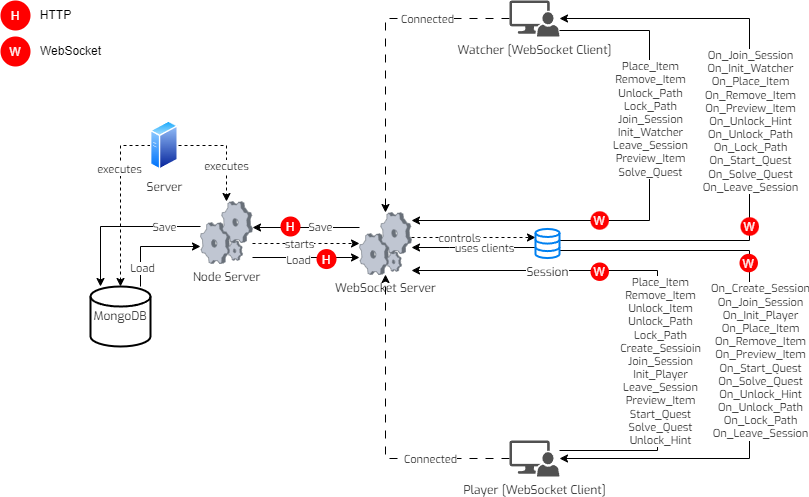
\includegraphics[width=1\linewidth]{content/pictures/Server-System.png}
\caption{Aufbau des Server (Quelle: eigene Darstellung)}
\label{fig:cm-server}
\end{figure}

Abbildung \ref{fig:cm-server} veranschaulicht den Aufbau des Serversystems. Der physische Server (in diesem Fall ein Laptop) betreibt dabei sowohl eine MongoDB-Datenbank als auch einen Node.js Server. Die MongoDB dient der persistenten Speicherung einzelner Spielsitzungen (Sessions). Der Node-Server bildet das zentrale Element der Serveranwendung. Er startet den WebSocket-Server, über den sich die Spielteilnehmer mit dem System verbinden.

Der WebSocket-Server übernimmt zudem die Verwaltung neuer Sessions. Auf Anforderung des Players wird eine neue Session generiert, der dieser anschließend automatisch beitritt. Ein Watcher kann über den WebSocket-Server ebenfalls einer existierenden Session beitreten. Die Kommunikation der einzelnen Clients erfolgt dabei ausschließlich über den Server, der die jeweiligen Informationen an die zugehörigen Session weiterleitet. Der Datenaustausch basiert auf dem zuvor beschriebenen WebSocket-Protokoll.

Beim Verlassen einer Session wird deren aktueller Zustand durch den WebSocket-Server gesichert. Dies geschieht über \ac{HTTP}-Anfragen an den Node-Server, der über definierte Endpunkte die Speicherung der Sitzungsdaten in der Datenbank vornimmt. Bereits gespeicherte Sessions können zu einem späteren Zeitpunkt erneut geladen werden. Senden sowohl Player als auch Watcher eine Beitrittsanfragen an den WebSocket-Server, wird über den Node-Server die entsprechende Session geladen und, sofern vorhanden, der Beitritt ermöglicht.

\section{Herausforderungen in der Umsetzung}\label{sec:difficulties}

Die Umsetzung einer Spielidee bringt im Verlauf des Entwicklungsprozesses häufig diverse Herausforderungen mit sich, die auf unterschiedliche Weise gelöst werden müssen. Auch im Rahmen dieser Arbeit traten mehrere Hürden auf, die es zu überwinden galt.

\subsection{Erste Schritte im Leveldesign}

Zu Beginn der Spielweltgestaltung wurde ein Ansatz gesucht, der eine effiziente und flexible Gestaltung der Umgebung ermöglicht, sodass im weiteren Verlauf der Fokus auf der Entwicklung der darin integrierten Rätsel liegen konnte. Zur Umsetzung dieses Vorhabens wurde das Unity-Package von \cite{alasl_autolevel_2022} näher untersucht.

Dieses Asset beinhaltet einen sog. \say{Level-Builder}, der auf Basis vorkonfigurierter Modelle aus einem Repository prozedural Spielwelten generiert. Abbildung \ref{fig:level_builder} zeigt dessen Anwendung in der Entwicklungsumgebung. Innerhalb eines vorgegebenen Rasters können einzelne Bauelemente ausgewählt und mit spezifischen Parametern versehen werden, etwa der Definition von Hohlräumen oder der Einbindung zusätzlicher Elemente aus weiteren Repositorys.

\begin{figure}[ht]
\centering
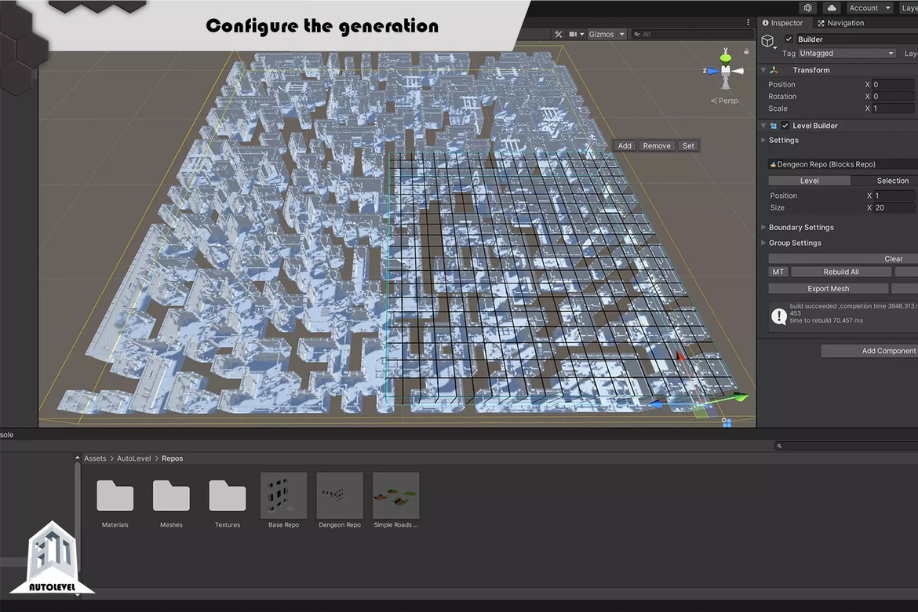
\includegraphics[width=1\linewidth]{content/pictures/FirstSteps00.png}
\caption{Level Builder Komponente (Quelle: \citealp{alasl_autolevel_2022})}
\label{fig:level_builder}
\end{figure}

Abbildung \ref{fig:level_builder_edit} veranschaulicht diesen Vorgang. Eine Teilfläche am oberen Rand des vom Level-Builder definierten Bereichs wurde über das zugehörige Konfigurationsmenü ausgewählt und kann nun mit spezifischen Anweisungen für die Generierung versehen werden. In diesem Fall erhält der markierte Bereich die Eigenschaft Empty, wodurch der Generator an dieser Stelle bewusst keinen Raum erzeugt. Auf diese Weise lässt sich die Struktur der Spielwelt gezielt beeinflussen und an konzeptionelle Anforderungen anpassen.

\begin{figure}[ht]
\centering
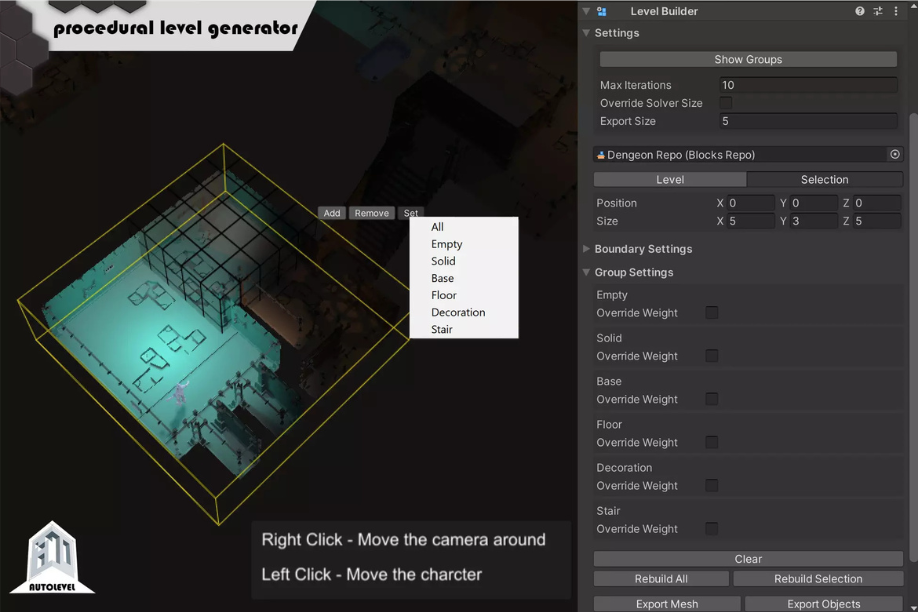
\includegraphics[width=1\linewidth]{content/pictures/FirstSteps01.png}
\caption{Level Builder Komponente (Quelle: \citealp{alasl_autolevel_2022})}
\label{fig:level_builder_edit}
\end{figure}

Um das Generieren der Spielwelt zu ermöglichen, muss zunächst ein Repository mit modularen \ac{3D}-Objekten erstellt werden, auf das der Generierungsalgorithmus zugreifen kann. Ein solches Repository besteht aus einzelnen, jeweils 1x1x1 Meter großen Bauelementen die über das in Abbildung \ref{fig:repository-generator} dargestellte Konfigurationsmenü zu größeren Einheiten zusammengesetzt werden können. Aus den sechs gezeigten Grundelementen lassen sich auf diese Weise vielfältige Kombinationen, bspw. 2x3 große Baustrukturen erzeugen, die ausschließlich vom Level-Builder automatisch in die Spielwelt integriert werden können.

\begin{figure}[ht]
\centering
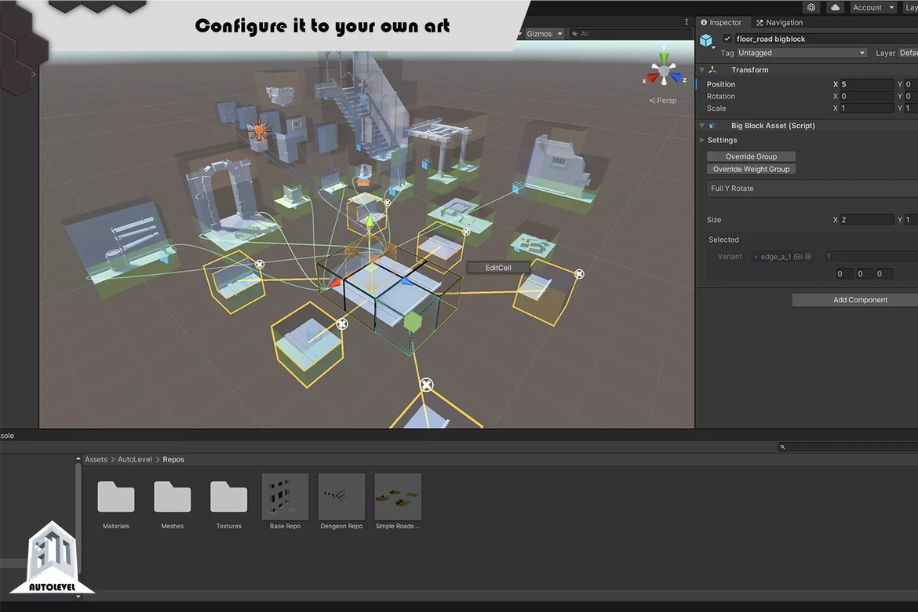
\includegraphics[width=1\linewidth]{content/pictures/FirstSteps02.png}
\caption{Level Builder Komponente (Quelle: \citealp{alasl_autolevel_2022})}
\label{fig:repository-generator}
\end{figure}

Das zuvor eingesetzte Paket setzt jedoch voraus, dass jedes strukturgebende \ac{3D}-Objekt in seine 1x1x1 Meter großen Basiselemente zerlegt wird. Für die Anpassung der Assets, die über den Unity Asset Store eingebunden wurden, wäre dieser Aufwand unverhältnismäßig hoch gewesen. Daher wurde nach einer alternativen Lösung gesucht, die mit bereits fertigen Strukturelementen wie Bodenplatten oder Wandmodulen arbeitet. \cite{mysticforge_low_2025} bietet einen Generator an, der für verschiedene Abschnittstypen, Kurven (links/rechts), zwei oder dreifache Kreuzungen sowie gerade Strecken, mehrere Varianten zur Verfügung stellt, aus denen automatisch eine zusammenhängende Spielwelt generiert werden kann. Zusätzlich besteht die Möglichkeit, vollständig vorbereitete Räume zu integrieren, in denen im späteren Verlauf Rätsel platziert werden können. Die vom Generator erzeugten Verbindungselemente zwischen diesen Räumen dienen dabei als Übergänge, durch die der Watcher den Player navigieren muss. Auch wenn dieser Generator bestimmte Größenanforderungen an die Modelle stellt, sind diese deutlich weniger granular als beim System von \cite{alasl_autolevel_2022} und beziehen sich auf funktionale Bauelemente wie komplette Wand- und Bodenstrukturen.

\begin{figure}[ht]
\centering
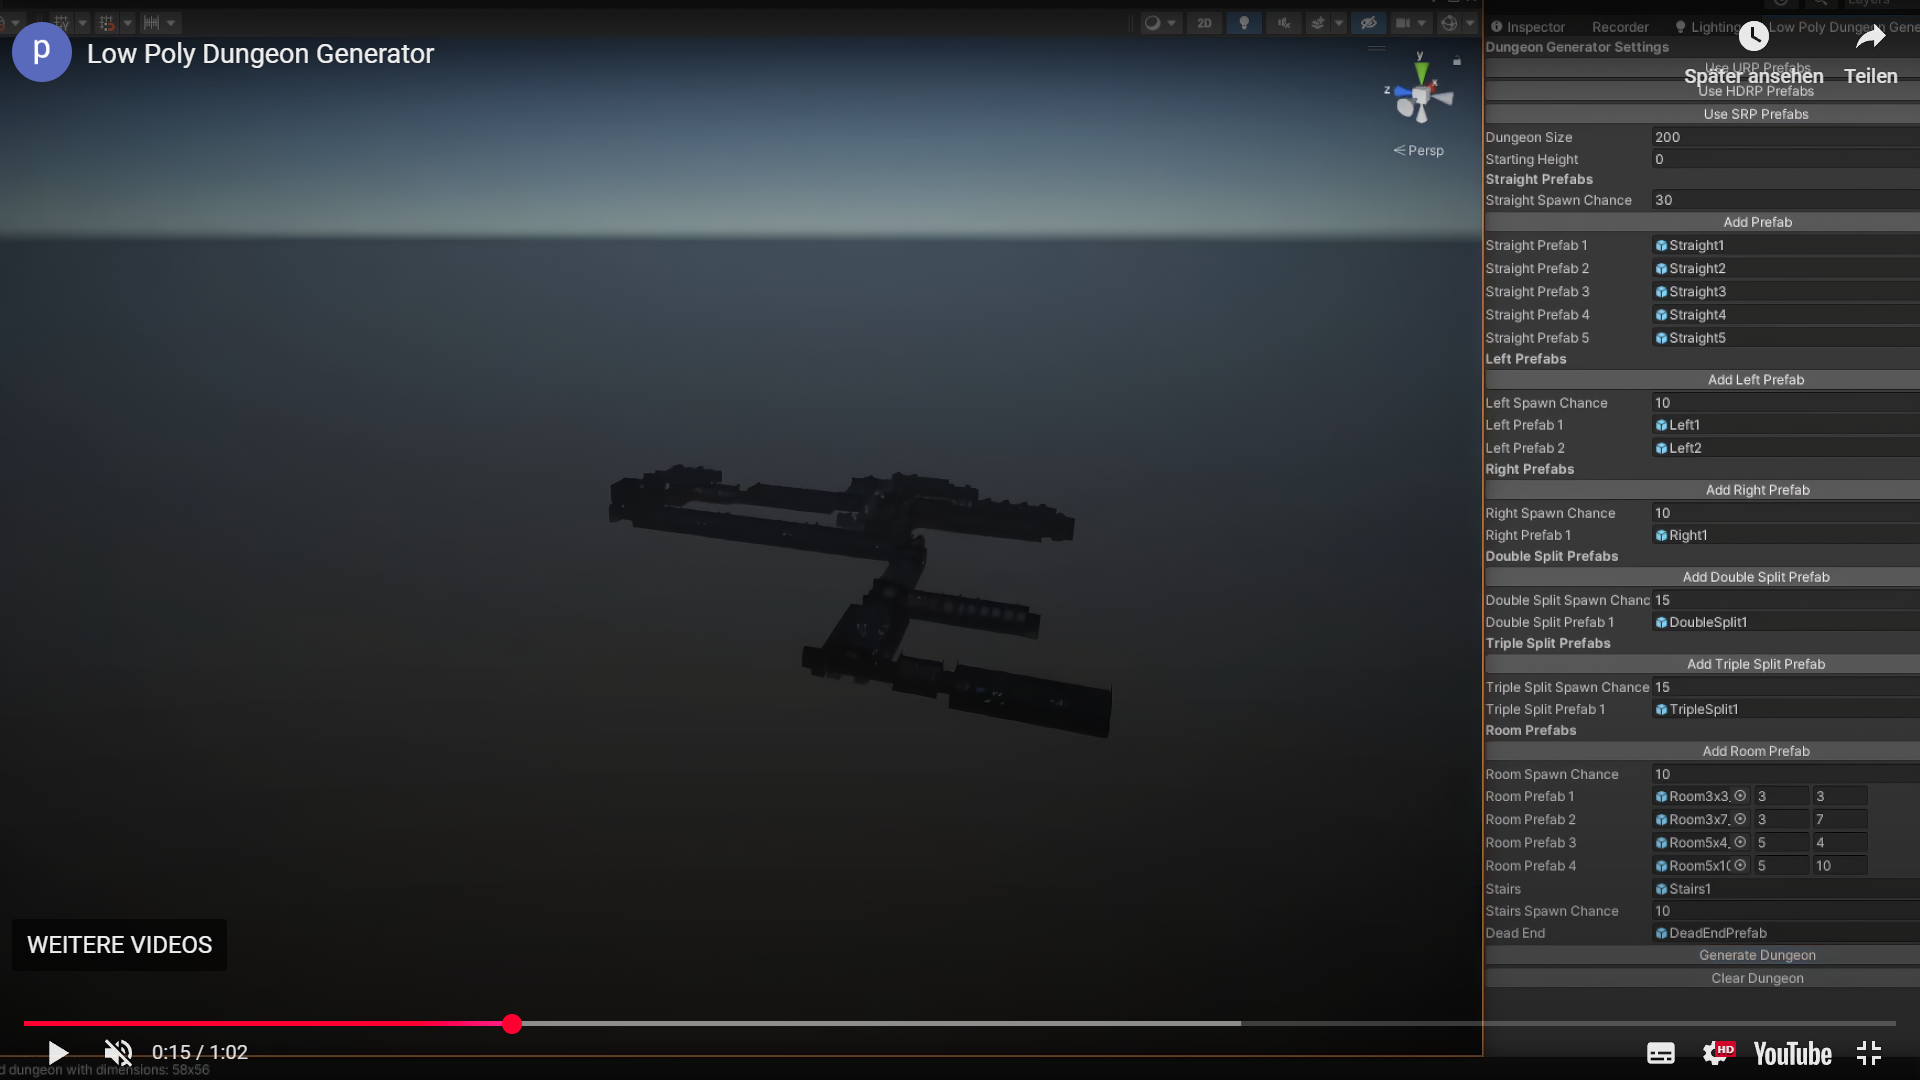
\includegraphics[width=1\linewidth]{content/pictures/FirstSteps03.png}
\caption{Low-Poly Dungeon Generator (Quelle: \citealp{past12pm_low_2024})}
\label{fig:dungeon-generator}
\end{figure}

Ein zentrales Problem des eingesetzten Generators besteht darin, dass die verschiedenen Strukturelemente in zufälliger Reihenfolge aneinandergereiht werden. Um dennoch eine kontrollierbare Struktur zu ermöglichen, wurde ein Element aus dem zuvor beschriebenen Generator-Konzept übernommen und zwar die Möglichkeit, spezifische Abfolgen von Bauelementen zu definieren. Damit konnte festgelegt werden, welche Module aufeinander folgen oder welchen Modulen bestimmte Elemente zwingend vorausgehen müssen. Abbildung \ref{fig:athaeck-dungeon-generator} zeigt im oberen Bereich die normgerecht erstellten Strukturelemente und im unteren Bereich die daraus generierten Übergänge zwischen den Räumen. Trotz dieser Erweiterung zeigt sich jedoch, dass das zugrunde liegende Zufallsprinzip in Kombination mit Wahrscheinlichkeitsverteilungen für die Auswahl bestimmter Module zu einer Unruhe im Layout führt. Die resultierenden Wege und Übergänge erwiesen sich daher für den intendierten Anwendungskontext als ungeeignet.

\begin{figure}[ht]
\centering
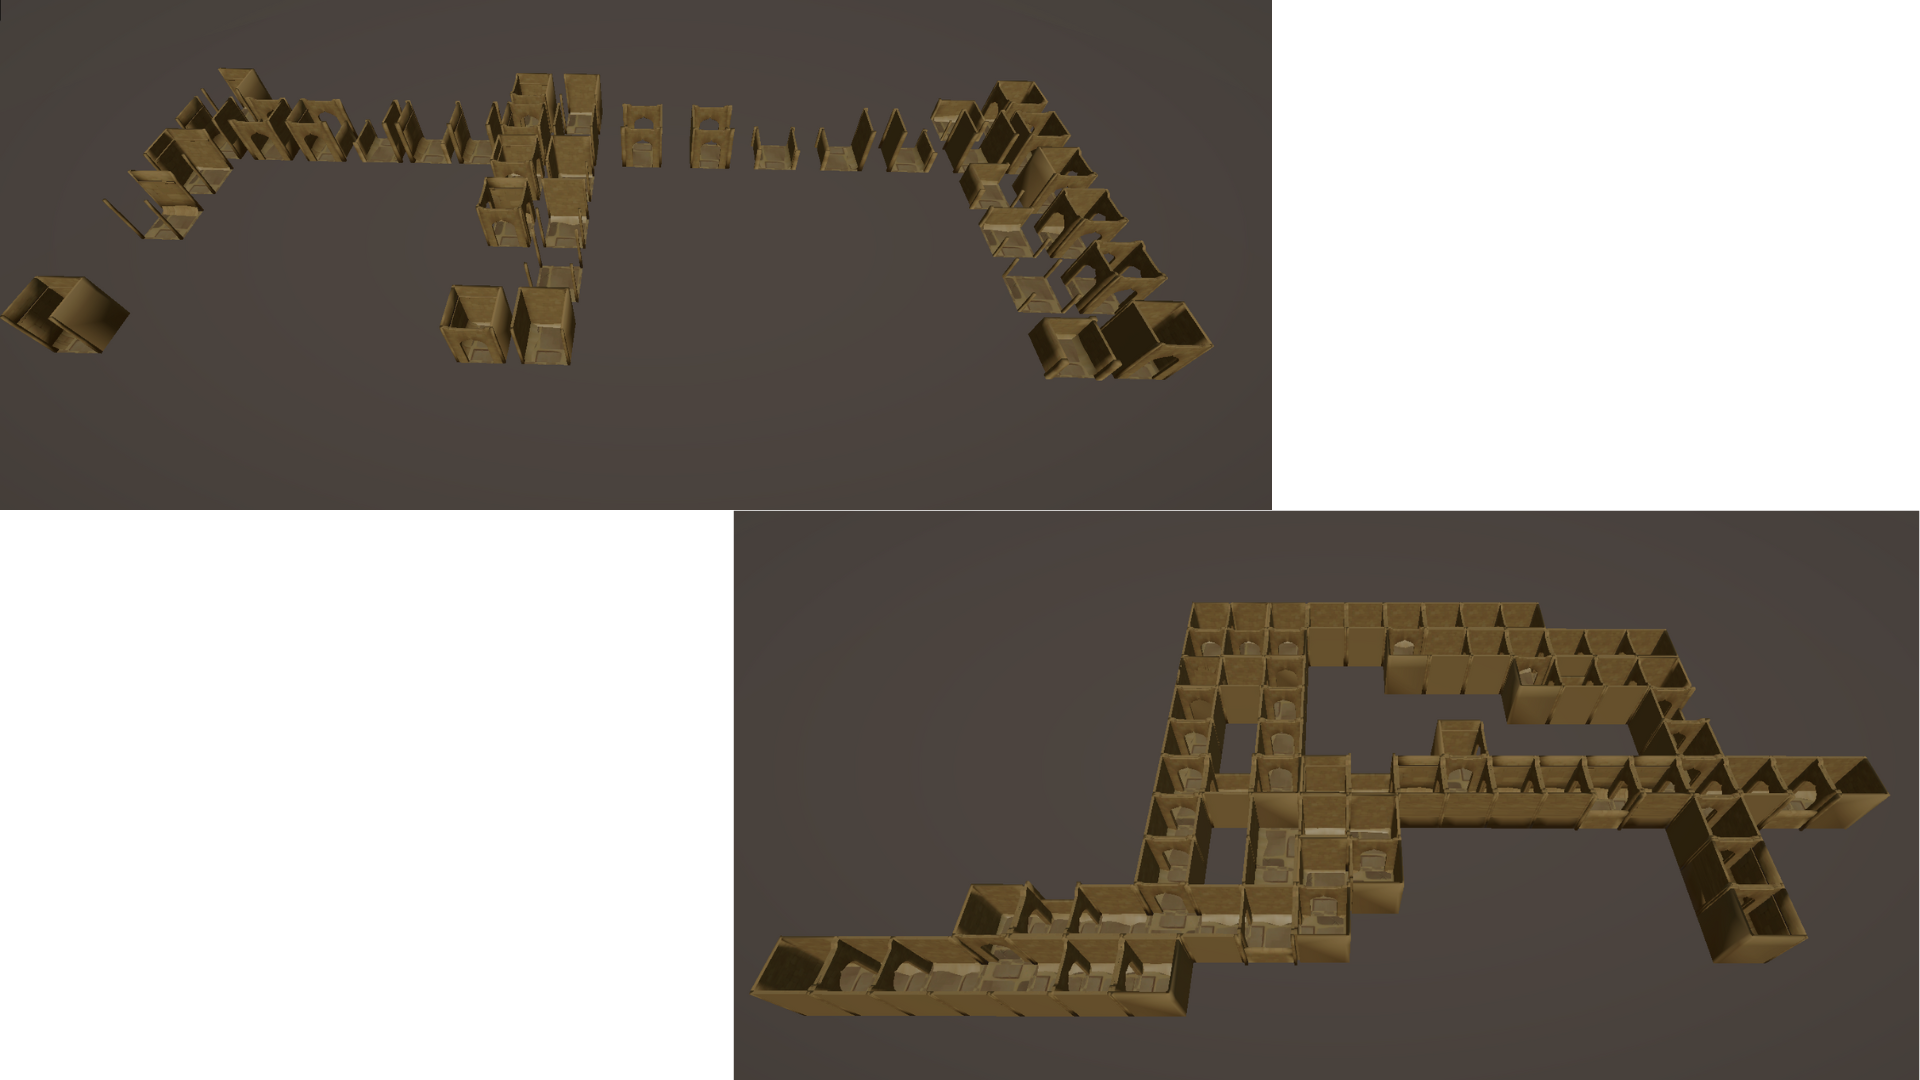
\includegraphics[width=1\linewidth]{content/pictures/FirstSteps06.png}
\caption{athaeck Dungeon Generator (Quelle: eigene Darstellung)}
\label{fig:athaeck-dungeon-generator}
\end{figure}

Trotz der letztlich verworfenen Umsetzung hatte der entwickelte Ansatz einen positiven Nebeneffekt. Da die einzelnen Strukturelemente an eine selbst definierte Größennorm angepasst werden mussten, konnte diese Norm im weiteren Verlauf auch auf zusätzliche, neu integrierte Assets übertragen werden. Dadurch wurde eine konsistente Maßstabsgrundlage für das gesamte Leveldesign geschaffen, was die Integration weiterer Elemente erleichterte und zur strukturellen Kohärenz der Spielwelt beitrug (vgl. Maßstäbe in Anhang \ref{sec:append_realisation_maßstaebe}; \nameref{sec:append_realisation_maßstaebe}).

\subsection{Physik-System von Unity}\label{sec:unity-physics-system}

Die zentrale Spielmechanik des Prototyps besteht im Lösen von Hindernissen durch das gezielte Platzieren von Objekten an definierten Positionen in der Spielwelt. In Teilen erfolgt die Validierung dieser Platzierungen über das Physiksystem von Unity. Jeder platzierbare Gegenstand ist mit einem Collider ausgestattet, der auf Kollisionen mit anderen Collider-Komponenten, bspw. dem des Player-Avatars, reagiert. Wie in den zuvor beschriebenen Beispielen des \say{QuestSolver} (vgl. Abschnitt \nameref{sec:quest-system}) oder des \say{PathActivator} (vgl. Abschnitt \nameref{sec:path-system}) beschrieben, prüfen diese Komponenten, ob ein Gegenstand innerhalb ihres eigenen Collider-Bereichs platziert wurde und lösen daraufhin entsprechende Spielereignisse aus (vgl. Abbildung \ref{fig:collision-sketch}). 

\begin{figure}[ht]
\centering
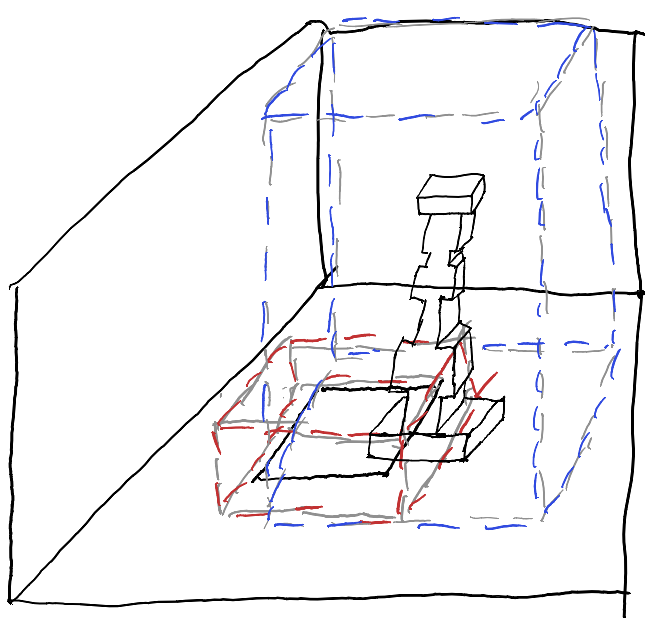
\includegraphics[width=.6\linewidth]{content/pictures/CollisionSketch.png}
\caption{Kollision zweier Collider in dem Raum, bei dem blau und rot sich kreuzen (Quelle: eigene Darstellung)}
\label{fig:collision-sketch}
\end{figure}

Sobald ein Gegenstand innerhalb des Zielbereichs eines anderen Colliders platziert wird, registriert das Physiksystem von Unity eine Kollision, welche in den entsprechenden Klassen verarbeitet werden kann. Das \say{Script lifecycle flowchart} von \cite{technologies_unity_2019} veranschaulicht diesen Ablauf. Nach dem Instanziieren eines neuen Knotens in der Spielwelt beginnt zunächst die Initialisierung der zugehörigen Skripte. Darauf folgt die Auswertung des Physiksystem, ehe der Ablauf über Input-Events zur Spiellogik übergeht.

Im Rahmen der Entwicklung traten jedoch Probleme beim Entfernen platzierter Objekte aus den zuvor genannten Zielradien der Collider auf. Der Lebenszyklus von Unity sieht vor, dass nach dem Entfernen eines Objekts keine weitere physikalische Berechnung für dieses durchgeführt werden (vgl. Diagrammabschnitt \say{OnApplicationQuit}). Für das System zur Lösung von Hindernissen, insbesondere im Hinblick auf die Aktivierung oder Deaktivierung bestimmter Pfade, stellt dies eine erhebliche Einschränkung dar.

Zur Lösung dieses Problems wurde eine Basisklasse entwickelt, die auf alle zur Laufzeit hinzugefügten und wieder entfernten Objekt angewendet wird. Im Gegensatz zur bisherigen Vorgehensweise, bei der ausschließlich das empfangende Objekt Kollisionen verarbeitete, wird nun auch der verursachende Gegenstand, selbst wenn er entfernt wird, aktiv in den Kollisionsprozess eingebunden.

\begin{figure}[ht]
\centering
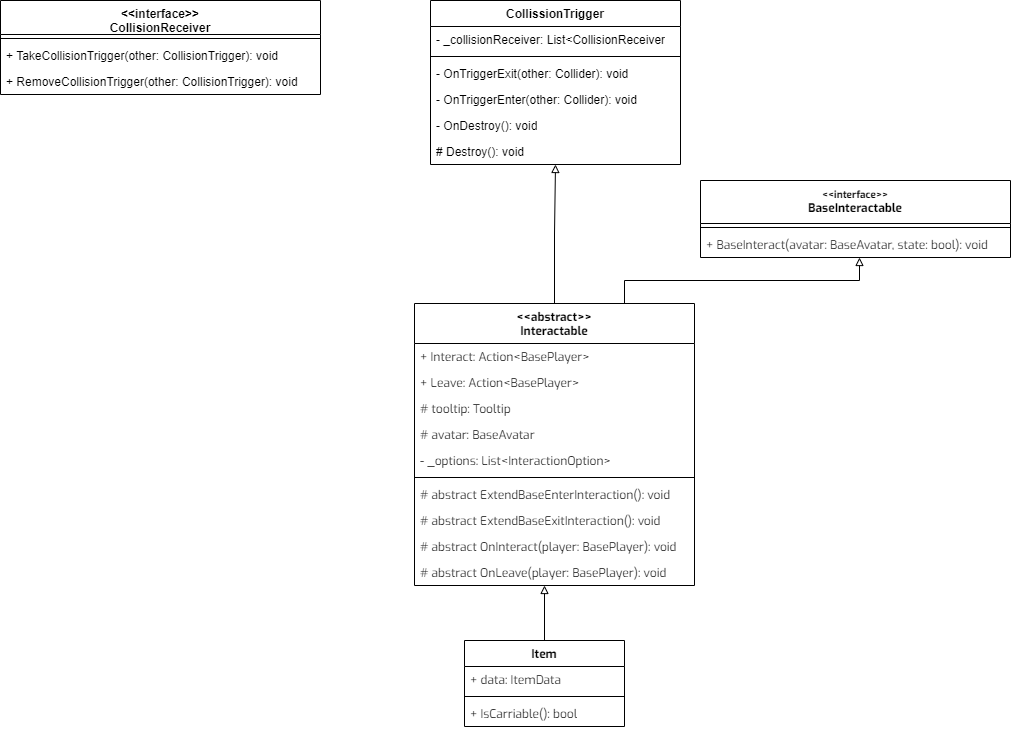
\includegraphics[width=1\linewidth]{content/pictures/CollisionSystem.drawio.png}
\caption{Neue Herangehensweise an Kollisionen (Quelle: eigene Darstellung)}
\label{fig:new-collision-system}
\end{figure}

Abbildung \ref{fig:new-collision-system} zeigt die neue Klassendefinition des \say{Verursachers} von Kollisionen, in der letzten Vererbungsstufe der \say{Item}-Klasse, das dem zu platzierenden Gegenstandsobjekt zugewiesen ist. Das zugehörige Empfänger-Interface wird, wie in Abbildung \ref{fig:new-collision-system-in-quests} dargestellt, von der Basisklasse \say{BasePlaceableActivator} implementiert.

\begin{figure}[ht]
\centering
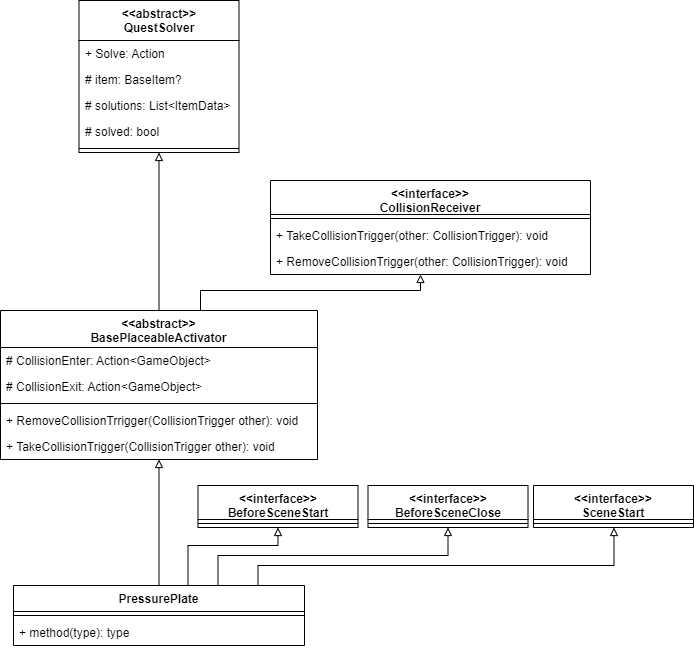
\includegraphics[width=0.8\linewidth]{content/pictures/Quest-Extension.drawio.png}
\caption{Kollisions-Empfänger im Quest-System (Quelle: eigene Darstellung)}
\label{fig:new-collision-system-in-quests}
\end{figure}

\subsection{Platzieren von Gegenständen außerhalb der Spielwelt}\label{sec:difficulties-placement}

Wie bereits erläutert, unterscheiden sich die Ansichten von Player und Watcher in bestimmten Bereichen der Spielwelt. Am Beispiel des Sicherheitsraums lässt sich exemplarisch ein zentrales Problem beim Platzieren von Gegenständen verdeutlichen.

Während sich der Player im Inneren des Gebäudes befindet, erhält der Watcher zusätzlich Einblick in einen angrenzenden Außenbereich. In diesem Außenbereich soll der Watcher einen zuvor gefundenen Stromgenerator platzieren. Da dieser Bereich für den Watcher sichtbar und zugänglich ist, erfolgt die Platzierung problemlos. Allerdings werden alle im Rahmen der Session platzierten Gegenstände synchronisiert, sie erscheinen sowohl für den Player als auch für den Watcher. Dies führt zu einem Problem. Der Player darf keine Gegenstände sehen, die sich in für ihn derzeit inaktiven oder unsichtbaren Bereichen befinden.

Zur Lösung dieses Problems wurden für jeden Bereich der Spielwelt spezifische Collider eingeführt. Diese sind dafür verantwortlich, platzierte Gegenstände kontextabhängig zu aktivieren oder zu deaktivieren, abhängig davon, ob der jeweilige Bereich für die jeweilige Rolle als aktiv gilt. Dabei greifen das zuvor angepasste System zur physikbasierten Kollisionsverarbeitung (vgl. Kapitel \nameref{sec:unity-physics-system}) und die im Kapitel  \nameref{sec:path-system} beschriebene Klasse PathCollider ineinander. Sie gewährleisten, dass sowohl Player als auch Watcher nur die für sie bestimmten Objekte in ihren jeweils aktiven Weltgebieten sehen können.

Dennoch treten in der Evaluation einzelne Grenzfälle auf, die im Kapitel \nameref{sec:prospect} näher behandelt werden.

\section{Probleme in der Umsetzung}

Für die Evaluation war ursprünglich vorgesehen, die Anwendung des Watchers mit einer \ac{AR}-Integration auszustatten. Ein zentrales Element funktionierender \ac{AR}-Anwendungen ist die stabile und zuverlässige Platzierung eines \ac{3D}-Objekts in den physischen Raum, sodass es aus der Sicht der Smartphone-Kamera den Eindruck erweckt, sich tatsächlich im realen Raum zu befinden.

Zur Realisierung dieser Funktionalität wurde das \say{Plane Detection}-Modul der ARFoundation eingesetzt. Um eine stabile Verankerung der Spielwelt zu gewährleisten, wurde zusätzlich ein \say{ARAnchor} auf einer erkannten Ebene (Plane) gesetzt. Dieser Anchor wird vom \say{AnchorManager} verwaltet, was eine zuverlässige Verortung im Raum ermöglichen soll.

Während der Entwicklung zeigte sich jedoch ein Problem. Die platzierte Spielwelt bewegte sich mit der Kamera mit, anstatt fest im Raum verankert zu bleiben. Dieses Verhalten ist ebenfalls im Unity-Forum dokumentiert (vgl. Beitrag von Howard258 in: \citealp{howard258_unity_2025}). Verschiedene Lösungsansätze, wie die Anpassung der Zuweisung zwischen Anchor und Plane oder das manuelle Verschieben des Weltobjekts in andere Hierarchien, blieben wirkungslos.

Ein weiterer Diskussionsbeitrag im Unity-Forum (\citealp{aardruss_ar_2023}) legt nahe, dass die verwendete Version der ARFoundation sowie die genutzte Unity-Editor-Version ursächlich für das fehlerhafte Verhalten sein könnten. Eine Herabstufung der Entwicklungsumgebung wurde aus zeitlichen und technischen Gründen jedoch nicht mehr umgesetzt. Außerdem hätte es potenziell auch zu Kompatibilitätsproblemen mit bestehenden Assets und Konfigurationen führen können.

Auch alternative Ansätze wie das \say{Image Tracking} wurden bewusst nicht verfolgt, Da sich der Watcher frei im physischen Raum bewegen soll, besteht bei dieser Methode das Risiko, dass das benötigte Referenzbild aus dem Sichtfeld verschwindet und damit die Spielwelt nicht mehr konkret dargestellt werden kann.